\documentclass[12pt,a4paper]{report}
%\documentclass[17pt]{extreport}
\usepackage[latin1]{inputenc}
\usepackage{ngerman}
\usepackage{makeidx,longtable,geometry,fancyhdr,color}
\usepackage{colortbl}
\usepackage[]{graphicx}
%-- dadurch werden zweizeilige Fussnoten einger�ckt
\usepackage[hang]{footmisc}
%-- refpage und bei dem Abk�rzungsverzeichniss steht die Seite auf der die Abk�rzung definiert wird
\usepackage[german,refpage]{nomencl}



\usepackage{enumitem}
\setlist{noitemsep,topsep=0.25cm}

\definecolor{dunkelgrau}{gray}{0.55}
\definecolor{hellgrau}{gray}{0.90}

\usepackage{listings}
\lstset{basicstyle=\scriptsize\ttfamily, numbers=left, numberstyle=\tiny, stepnumber=1,numbersep=10pt, firstnumber=1, backgroundcolor=\color{hellgrau}, frame=shadowbox, rulesepcolor=\color{dunkelgrau},
framesep=5pt, framerule=0.75pt, captionpos=b, breaklines=true, breakatwhitespace=false, escapeinside={!*}{*!}}

\renewcommand{\lstlistlistingname}{Quellcode Verzeichnis}
\renewcommand{\lstlistingname}{Quellcode}


% variable referenzennamen
\usepackage[german]{varioref}
\labelformat{lstlisting}{Quellcode~#1}
\labelformat{chapter}{Kapitel~#1}
\labelformat{section}{Abschnitt~#1}
\labelformat{subsection}{Unterabschnitt~#1}
\labelformat{subsubsection}{Unterunterabschnitt~#1}
\labelformat{paragraph}{Absatz~#1}
\labelformat{subparagraph}{Unterabsatz~#1}
\labelformat{figure}{Abbildung~#1}
\labelformat{table}{Tabelle~#1}
\labelformat{footnote}{Fussnote~#1}







%----Fuer Quellenangaben
\usepackage[square]{natbib}
\citestyle{natdin}
\bibliographystyle{natdin}





\usepackage{hyperref}
\hypersetup{% �=\304; �=\326; �=\334; �=\344; �=\366; �=\374; �=\377
  pdftitle={Provirent - Dokumentation},
  pdfauthor={Philipp Schneider},
  pdfcreator={Creator Philipp Schneider},
  pdfproducer={Producer Philipp Schneider},
  pdfsubject={},
  pdfkeywords={},
  colorlinks=false,   
  pdfpagemode=true,
  breaklinks=true,
  linkcolor = black, % blue
  anchorcolor=black % green
}


\pagestyle{fancy}
\renewcommand{\chaptermark}[1]{\markboth{#1}{}}
\renewcommand{\sectionmark}[1]{\markright{\thesection\ #1}}
\fancyhf{} % delete current setting for header and footer

\fancyhead[L]{\bfseries\rightmark}
\fancyhead[R]{}
\fancyfoot[C]{\bfseries\thepage}
\fancyfoot[L]{\bfseries\leftmark}
\fancyfoot[R]{\bfseries \footnotesize Provirent-Doku}

\renewcommand{\headrulewidth}{0.5pt}
\renewcommand{\footrulewidth}{0pt} 
\addtolength{\headheight}{2.5pt} % make space for the rule
\fancypagestyle{plain} {%
	\fancyhead{} % get rid of headers on plain pages
	\renewcommand{\headrulewidth}{0pt} % and the line
} 

%-- Index
\makeindex
\renewcommand{\indexname}{Stichwortverzeichnis} 

%--AbkuerzungsVerzeichnis
\renewcommand{\nomname}{Abk�rzungsverzeichnis}
\makenomenclature

%-- Zweilzeilig zum besseren Korrekturlesen 
%\usepackage{setspace}
%\doublespace      % doppelzeilig
%\onehalfspacing  % anderthalbzeilig

%hier werden die trennungen f�r spezielle W�rter definiert
\hyphenation{
Hal-lo
}

\begin{document}
%------ Begin des Dokumentes ------ 
   	\setlongtables
		\definecolor{Gray}{gray}{0.8}
 		\newcolumntype{E}{|>{\columncolor{Gray}[\tabcolsep]}c|}
 		\newcolumntype{A}{|>{p{8cm}\columncolor{Gray}[\tabcolsep]}l}
 		\newcolumntype{B}{|>{\columncolor{Gray}[\tabcolsep]}c|}
	 	\newcolumntype{C}{|>{\columncolor{Gray}[\tabcolsep]}c|}


%====================================
%\begin{titlepage}
\begin{center}
  {\large{\textsc{Projektarbeit}}}
  \\
  \vspace*{4.5cm}
  {
 \Huge{\textsc{provirent} \\[1cm]
 
  ---}
  }
%\newfont{\cminch}{cminch scaled 500}
%\textsc{\cminch{PROVIRENT}}
  \\
  \vspace{0.5cm}
  \Large{\textsf{\textbf{Prof}essional \textbf{Vi}deo \textbf{Rent}al Software}}
  \\
  \vspace*{7.5 cm}
\textsf{
    \begin{large}
    \begin{tabular}{ll}
      Student: & Stefan Forstner\\
      Student: & Remo Griesch\\
      Student: & Philipp Schneider\\
      Fachbereich: & Automatisierung und Informatik \\
      Fachrichtung: & Kommunikationsinformatik \\
      Betreuer: & Prof. Dr. Sigurd G�nther\\
      Abgabedatum: & 20. Dezember 2005
    \end{tabular}
  \end{large}
  }
\end{center}
\end{titlepage}



%\renewcommand{\abstractname}{Abstract}
\abstract Hier folgt eine kurze Zusammenfassung des Themas (ca. 5~
Zeilen).



\chapter*{Vorwort}







\tableofcontents

%\addcontentsline{toc}{chapter}{AbbildungsVerzeichnis}
%\listoffigures
%\addcontentsline{toc}{chapter}{TabellenVerzeichnis}
%\listoftables
%\addcontentsline{toc}{chapter}{Quellcodes}
%\lstlistoflistings
%====================================
\chapter{Einf�hrung} \label{sec:Einfuehrung}



\section{Grundlegendes} \label{sec:Grundlegendes}



\subsection{Betreuender Professor}
%===========================================
Hochschule Harz \\
Prof. Dr. Sigurd G�nther \\
Friedrichstr. 57- 59 \\
38855 Wernigerode \\
sguenther@hs-harz.de
%===========================================
\subsection{Studenten}
%===========================================		
\begin{tabular}{rrr}
	Remo Griesch							& Stefan Forstner 				& Philipp Schneider 				\\
	Strasse										&	Strasse der Jugend 22  	& Kastanienring 16				\\
	Ort												&	04880 Dommitsch					& 04316 Leipzig							\\[0.4cm]
	Romeodied@gmx.de					&	fossiossi@web.de				& provirent@phil-schneider.de \\
	
	
	
\end{tabular}		
			
\subsection{Kapitelarbeit} \label{sec:Kapitel}

\subsubsection{Remo Griesch}
\ref{sec:tech-Entwicklungsumgebung} \vpagerefrange{sec:tech-Entwicklungsumgebung}{sec:tech-Entwicklungsumgebung-ende};

\ref{sec:tech-Benutzerschnittstellen} \vpagerefrange{sec:tech-Benutzerschnittstellen}{sec:tech-Benutzerschnittstellen-ende};

\ref{sec:impl-Entwicklungsumgebung}  \vpagerefrange{sec:impl-Entwicklungsumgebung}{sec:impl-Entwicklungsumgebung-ende};

\ref{sec:impl-Benutzerschnittstellen}  \vpagerefrange{sec:impl-Benutzerschnittstellen}{sec:impl-Benutzerschnittstellen-ende}

\subsubsection{Stefan Forstner}
\ref{sec:tech-WebAnwendungen} \vpagerefrange{sec:tech-WebAnwendungen}{sec:tech-WebAnwendungen-ende};

\ref{sec:tech-Persistenzschichten}  \vpagerefrange{sec:tech-Persistenzschichten}{sec:tech-Persistenzschichten-ende};

\ref{sec:impl-WebAnwendungen} \vpagerefrange{sec:impl-WebAnwendungen}{sec:impl-WebAnwendungen-ende};

\ref{sec:impl-Persistenzschichten}  \vpagerefrange{sec:impl-Persistenzschichten}{sec:impl-Persistenzschichten-ende}

\subsubsection{Philipp Schneider}
\ref{sec:Einfuehrung} \vpagerefrange{sec:Einfuehrung}{sec:Einfuehrung-ende};

\ref{sec:KonzepteundAufbau} \vpagerefrange{sec:KonzepteundAufbau}{sec:KonzepteundAufbau-ende};

\ref{sec:tech-Versionsverwaltung}  \vpagerefrange{sec:tech-Versionsverwaltung}{sec:tech-Versionsverwaltung-ende};

\ref{sec:impl-Versionsverwaltung}  \vpagerefrange{sec:impl-Versionsverwaltung}{sec:impl-Versionsverwaltung-ende}

\newpage
\section{Dokumentationsbeschreibung} \label{sec:Dokumentationsbeschreibung}
Im ersten Kapitel soll die Frage gekl�rt werden, wie es zu diesem Projekt kam. Dabei sollen erste Ideen zu diesem Projekt erl�utert und die Zielsetzung und die m�glichen Einsatzbereiche beschrieben werden.
Im zweiten Kapitel wird der Aufbau der Software mit den einzelnen Modulen beschrieben werden. Dabei sollen sowohl Ideen, Visionen und realisierbare Aufgaben detalliert erl�utert werden. zum Schluss dieses Kapitels...


Konzepte und Aufbau\\
-Aufbau des Projektes\\
-geplante Module und Versionen\\

Technologien\\
-Versionsverwaltung (CVS,SVN)\\

Implementierung mit Subversion als Versionsverwaltung\\


\textbf{\emph{Hier muss eine Beschreibung der anderen Abschnitte erfolgen.}}





















\section{Motivation} \label{sec:Motivation}
Im Rahmen des Studiums an der Fachhochschule Harz in Wernigerode muss jeder Student des Studiengangs Kommunikationsinformatik eine Projektarbeit abgeben. Dies bedeutet, da� der Student eine Aufgabe (meist Programmieraufgabe) alleine oder in einem kleinen Team bew�ltigen muss. Die Professoren der Hochschule bieten dabei viele interessante Projektarbeiten an, sind jedoch auf offen f�r eigene Vorschl�ge der Studenten.\\
Da schon in den Teamprojekten\footnote{Auch das Teamprojekt ist Bestandteil des Studiums. Beim Teamprojekt m��en mehrere Studenten (7-15) gemeinsam eine Programmieraufgabe umsetzen.} \emph{Labmin}\footnote{\url{http://labmin.de.vu}} und \emph{German Team Sony Aibo}\footnote{\url{http://www.der-baer.com/projects.htm}} eine interessante Aufgabe von den Studenten gel�st wurde, sollte das dort erlernte Wissen vertieft und weiter ausgebaut werden.


\section{Ideen zur Projektarbeit} \label{sec:Ideen}
\subsection{Tippspiel}\label{sec:Tippspiel}
Die erste Idee dieser Projektarbeit war die Umsetzung eines Tippspiels in Java, passend zu den damaligen Fussball-Europameisterschaft in Portugal. Diese Idee wurde im JavaMagazin\footnote{\citep{Frotscher2004}\citep{Frotscher2004a}\citep{Frotscher2004b}} in mehreren Ausgaben aufgegriffen und verschiedene Ansatzm�glichkeiten diskutiert. Die Idee unseres Tippspiel war dabei eine Webanwendung mit Datenbankanbindung. Nutzer dieses Systems sollten sich in verschiedenen Tippgemeinschaften, mit je einem Tippgemeinschaftverwalter, zusammen tun und gemeinsam die EM 2004 tippen. Das Tippspiel sollte jedoch nicht nur auf die EM 2004 zugeschnitten sein, sondern auch f�r andere Fu�ballereignisse tauglich sein. Zus�tzlich kam von unserer Seite die Idee, eine Webanwendung zur Verwaltung der Bundesligaergebnisse. Ein Tippspiel System sollte dann auf diese Daten zur�ckgreifen und so ein Bundesligatippspiel darstellen k�nnen.\\
Dieser Gedanke wurde jedoch aus verschiedenen Gr�nden verworfen. Zum einen war es nicht unsere Idee, sondern die des Javamagazin's und zum anderen wussten wir nicht sofort was bei diesem System alles zu realisieren war. Die grobe Funktionsweise war allen klar, jedoch fehlte bei diesem System das gewisse etwas. 
%===========================================
\subsection{Videosoftware} \label{sec:Videosoftware}
Da jeder von uns schon einmal ein Video in einer Videothek ausgeliehen, kam uns der Gedanke einer Onlinevideothek. Solche Videotheken gibt es mittlerweile schon wie bspw. Amango\footnote{\url{http://www.amango.de}}, Netleih\footnote{\url{http://www.netleih.de}},  Invdeo\footnote{\url{http://www.invdeo.de/}} und Verleihshop \footnote{\url{http://www.verleihshop.de}}. Bei genauer Betrachtung dieser Onlinevideotheken, fragten wir uns wie solch eine Videothek technisch funktioniert. Da wir gerade auf der Suche nach einem idealen Projekt waren, hatten wir damit eins gefunden.\\
Es solle versucht werden eine Online-Videothek mit entsprechenden Modulen zu realisieren.



\section{Zielsetzung und Einsatzbereich} \label{sec:Zielsetzung}
\textbf{Muss noch �berarbeitet und zusammengefasst werden}\\
Zielsetzung dieses Projektes ist dabei Erfahrung mit verschiedenen neuen Technologien zu sammeln und selbst�ndig an einem Projekt zu arbeiten. Sowohl die eigene Gedanken, Ideen, Planung und auch Realisierung dieses Projektes sollten uns auf eine sp�tere Eigenverantwortung im Berufsleben vorbereiten. Das Projekt sollte dabei keine vollst�ndige und fehlerfreie Implementierung darstellen. Uns war bewu�t, dass wir nur einen einfachen Prototypen einzelner Module realisieren k�nnten.\\
Diese Software ist sowohl f�r kleine als auch f�r grosse Unternehmen gedacht. Dabei ist es unwichtig, ob es sich um eine reine OnlineVideothek oder um eine richtige Videothek, die jetzt auch per Versand ihre Videos verleihen m�chte, handelt. Durch weitere Module kann die Software so erweitert werden, dass die Software auch f�r eine richtige Videothek geeignet ist. 
%===========================================



\label{sec:Einfuehrung-ende}
%====================================
\chapter{Konzepte und Aufbau} \label{sec:KonzepteundAufbau}
%===========================================
\section{Aufbau}\label{sec:Aufbau}
\subsection{Beschreibung des Gesamtsystems}\label{sec:ersteGedanken}
Bei einer klassischen Videothek besucht der Kunde das Ladengesch�ft der Videothek und st�bert dabei nach Videos, die er gerne an diesen Abend schauen m�chte. Dabei muss die Videothek eine m�glichst gr��e Ladenfl�che besitzen um die Videos dem Kunden zu pr�sentieren. Nachdem der Kunde sich f�r ein Video entschieden hat, nimmt er entweder die leere Verpackung oder ein Plastikschild mit einer Nummer zum Verleihschalter der Videothek. Nachdem der Kunde seine Kundenkarte vorzeigt und durch sein Passwort oder seine Unterschrift verifiziert wurde, sucht der Mitarbeiter anhand einer Nummer in der Leerverpackung oder des Plastikschilds das entsprechende Video heraus, markiert dieses Video im System und gibt es dem Kunden. Dies ist der klasische Ablauf in einer Videothek.\\
Bei einer Online-Videothek kann der Kunde, durch den Versand der Videos, keine Videos f�r den gleichen Abend ausleihen. Er ist gezwungen, sich einige Tage vorher f�r ein oder mehrere Videos zu entscheiden. Der Ablauf unterscheidet sich von einer klasischen Videothek. Der Kunden "`besucht"' die Webseite der Videothek und sucht im Angebot nach Filmen die er sich ausleihen m�chte. Nachdem die Verf�gbarkeit �berpr�ft wurde, legt er Videos in seinem Warenkorb ab. Durch Eingabe seines Benutzernamens und das zugeh�rige Passwort wird der Kunde verifiziert. In dem Lager der Videothek nimmt ein Mitarbeiter die Bestellung �ber einen Monitor oder eine ausgedruckte Liste entgegeben und bearbeitet die Bestellung. Dabei sucht dieser die Videos f�r den Kunden heraus, nimmt die Videos in das System auf und versendet die Videos zu dem Kunden per Post. Der Kunde erh�lt seine gew�nschten Videos, kann diese sich anschauen und schickt diese nach einer bestimmten Zeit an die Videothek zur�ck.\\
Das hier gew�nschte System soll dabei eine komplette Videothek ersetzen. Die Online-Videothek ben�tigt nur noch ein Lager f�r die zu verleihenden Videos und wenige Mitarbeiter f�r den Versand der Videos und die Verwaltung der Videothek. Die Software wird  dabei wie in \vref{fig:erstegedanken} zu sehen ist, von zwei verschiedenen Personenkreisen benutzt, dem Kunden und dem Mitarbeiter. Der Kunde kann die in der Abbildung dargestellten Aktionen ausf�hren, wie bspw. betrachten und bestellen von Videos. Der Mitarbeiter kann dabei das System verwalten und Bestellungen der Kunden bearbeiten.\\
%===========================================
\begin{figure}[p]
	\rotatebox{90}{
		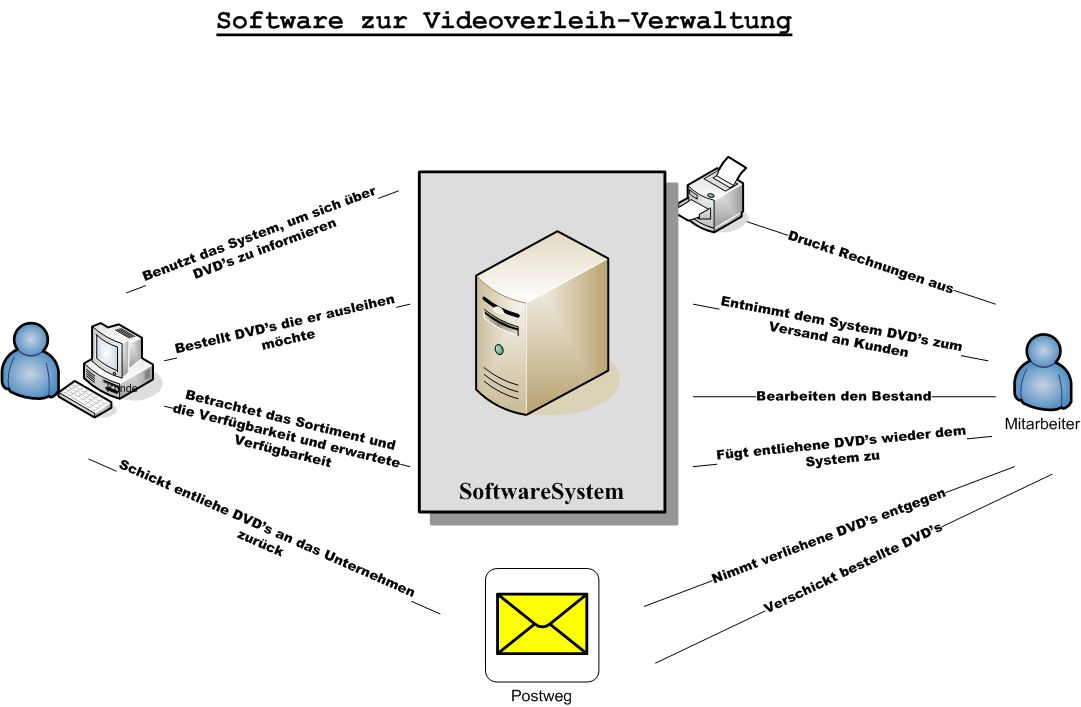
\includegraphics[scale=0.65]{images/erste-gedanken.jpg}
	}
	\caption{Erste Gedanken zu der Videosoftware}
	\label{fig:erstegedanken}
\end{figure}
%===========================================
Nach einiger �berlegung wurde festgestellt, das die Software aus drei anstatt zwei Modulen bestehen muss, wie in \vref{fig:dreimodule} zu sehen ist. Bei den Mitarbeitern der Online-Videothek muss in Verwaltung und Versand/Lagen unterschieden werden, da diese unterschiedlichen Aufgaben von unterschiedlichen Mitarbeitern bearbeitet werden. Das \textbf{Kundenmodul} ist die Internetpr�senz der Videothek und repr�sentiert das Unternehmen nach aussen. Auf dieser dynamischen Webseite kann der Kunde die vorhanden Videos durchst�bern und detaillierte Informationen zu den Videos erhalten. Nach erfolgreicher Anmeldung im System kann der Kunde die Verf�gbarkeit des jeweiligen Videos kontrollieren und auf Wunsch Videos ausleihen. In einem zus�tzlichen Men�punkt kann er seine bestellten Videos betrachten und sich ggf. Rechnungen ausdrucken. Das \textbf{Versandmodul} stellt die ben�tigte Software f�r das Lager und den Versand zur Verf�gung. Mit deren Hilfe kann ein Mitarbeiter der Online-Videothek Videos f�r den Versand vorbereiten. D.h. der Mitarbeiter bekommt eine Liste mit Bestellungen von Kunden (elektronisch oder auf Papier) und arbeitet diese ab. Damit der Mitarbeiter nicht jedes mal die Kundennummer und Nummern der Videos eintippen muss, wird seine Arbeit durch Barcodes und Barcodescanner unterst�tzt. Mit dessen Hilfe markiert er Videos f�r einen bestimmten Kunden und eine bestimmte Bestellung und versendet diese. Dem System teilt der Mitarbeiter dadurch mit, das bestimmte Videos nicht mehr verf�gbar sind und von einem bestimmten Kunden ausgeliehen wurde. Rechnungen, Versandetiketten und eventuelle Lieferscheine werden dabei automatisch mit Hilfe eines Druckers erstellt. Zus�tzlich bietet das Versandmodul die M�glichkeit, zur�ckgekommene Videos der Kunden wieder in das System aufzunehmen. Somit wurde das Video wieder vom Kunden zur�ckgegeben und es kann im System als vorhanden/ausleihbar markiert werden oder gleich an den n�chsten Kunden weitergeschickt werden. Das \textbf{Verwaltungsmodul} hilft den Mitarbeitern in der Verwaltung bei der Organisation der Online-Videothek. Es k�nnen Kundendaten und Rechnungen betrachtet und ggf. gedruckt werden. Das Videosortiment kann bearbeitet und inhaltliche �nderungen (z.B. Sonderangebote) an dem Kundenmodul vorgenommen werden. Weiterhin besteht die M�glichkeit ausf�hrliche Reports \& Statistiken zu erstellen und zu betrachten.\\
%===========================================
\begin{figure}[tbp]
	\centering
	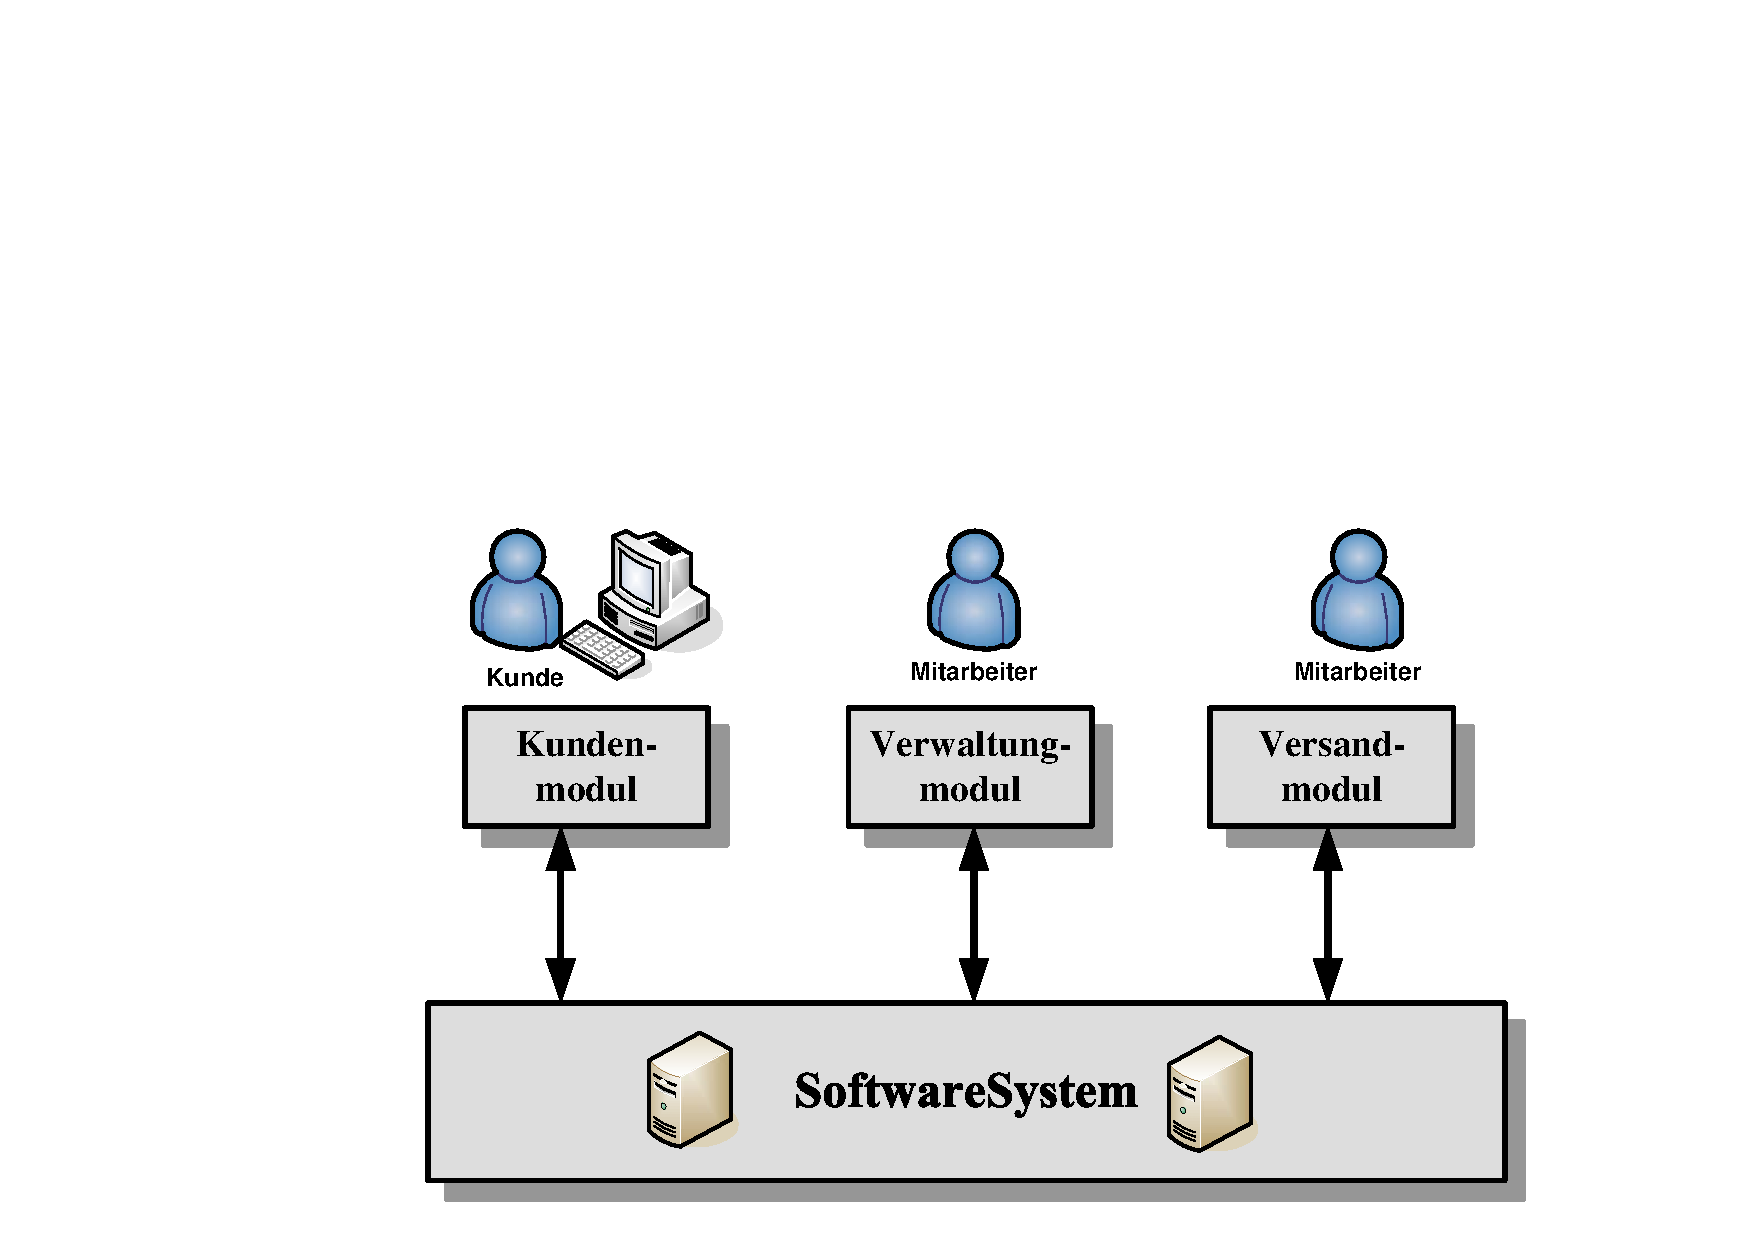
\includegraphics[scale=0.65]{images/dreimodule.pdf}
	\caption{Die drei Module der Software}
	\label{fig:dreimodule}
\end{figure}
%===========================================


%===========================================
\subsection{das Kundenmodul im Detail} \label{sec:Kundenmodul}
Das Kundenmodul ist das wichtigste Element der Anwendung, denn dieses Modul wird vom Kunden verwendet und dieser bestimmt �ber Erfolg oder Misserfolg der Online-Videothek und damit �ber die Anwendung. Das Kundenmodul wird, wie bereits erkl�rt, als Webanwendung entwickelt. Somit muss der Nutzer keine spezielle Software auf seinem Rechner verwenden und kann die Software somit �berall verwenden. Grunds�tzlich wird bei der Anwendung zwischen zwei verschiedenen Kundengruppen unterschieden: dem \emph{Interessenten} und dem \emph{angemeldeten Kunden}. Ein \emph{Interessent} ist ein Websurfer, der sich �ber das Angebot der Online-Videothek interessiert, ohne bisher ein Video ausgeliehen zu haben. Ist der Interessent von dem Angebot �berzeugt und m�chte ein Video ausleihen, muss er sich im System registrieren. Dazu geh�rt neben einem Benutzernamen und Passwort auch seine vollst�ndige Adresse, f�r den Versand der Videos bzw. Rechnungen, und seine Bankverbindung bzw. Kreditkartendaten, f�r die Bezahlung. Ist Kunde in das System eingeloggt, ist er ein angemeldeter Kunde. Je nach Kundengruppe pr�sentiert sich die Webseite mit anderen Funktionalit�ten. Zuerst sollen die Funktionen und M�glichkeiten eines Interessenten erkl�rt werden. Der Interessent hat kann sich auf der Webseite der Online-Videothek sowohl �ber das Angebot an Videos, als auch �ber die Online-Videothek informieren. �ber verschiedene Webseiten erh�lt er Einblick in die f�r ihn interessante Funktionsweise der Online-Videothek und allgemeinen Daten, wie Impressum, Kontaktdaten und Allgemeine Gesch�ftsbedingungen. �ber eine intelligente Suche und Navigationselementen kann er nach Videos suchen bzw. st�bern. Die Videos sind kategorisiert bzw. geordnet. Der Interessent kann auch detaillierte Informationen �ber einzelne Filme erhalten. Dabei kann er sich �ber die Features des Filmes informieren, Kommentare bzw. Bewertungen lesen und �hnliche Filme betrachten. Die dabei verwendete Suche wird als inteligente Suche bezeichnet, weil diese Suche auch �hnliche bzw. verwandte Filme findet und  sowohl im Titel, als auch in der Beschreibung der Filme nach dem Stichwort sucht. Es k�nnte auch realisiert werden, das die Suchergebnisse nach Trefferquoten geordnet werden bzw. das Suchfeld automatisch das Wort nach h�ufigen Suchbegriffen erg�nzt.\\
Ist der User eingeloggt hat er die gleiche Funktionsweise wie ein Interessent, nur mit erweiterten Funktionen. In der Ergebnissliste der Suche oder der Anzeigeliste der Kategorien, welche beide gleich aufgebaut sind, befinden sind neben jedem Video Elemente zum bestellen und zum �berpr�fen der Verf�gbarkeit. Jedes Video, also jeder Film, ist in einer gewissen Anzahl vorhanden. Mit Hilfe der �berpr�fung der Verf�gbarkeit kann der Kunde �berpr�fen, ob noch ein Video dieses Filmes f�r ihn zum Ausleihen vorhanden ist, bzw. wann das n�chste Video wieder verf�gbar ist. Je nach Status der Verf�gbarkeit kann der Kunde das Video in seinem Warenkorb legen und damit ausleihen, oder vormerken lassen. Bei einer Vormerkung wird er entweder per Email informiert, dass das Video vorhanden ist, oder das Video wird schnellstm�glich an den Kunden versendet. Hat der Kunden Videos in seinen Warenkorb abgelegt, kann dieser am Ende seiner Bestellung zur Kasse gehen und somit die Videos ausleihen. Weiterhin hat der Kunde die M�glichkeit eine so genannte \emph{Wunschliste} zu Erstellen. Diese Liste kann eine bestimmte Anzahl an Videos anschauen, die der Kunde schauen m�chte. Das System arbeitet diese Liste automatisch ab, indem es dem Kunden eine bestimmte Anzahl an Videos mit einmal zusendet und bei R�cksendung durch den Kunden die n�chsten Filme automatisch an den Kunden sendet. Somit hat der Kunden z.B. die M�glichkeit 50 Filme zu bestimmen, die er gerne anschauen m�chte. Das System sendet ihm immer zwei Filme mit einmal zu, die er sich anschauen kann. Sendet er diese zwei Filme zur�ck, bekommt er die n�chsten zwei Filme, bis die Liste abgearbeitet wurde. Weiterhin bietet das Kundenmodul dem Kunden die M�glichkeiten, �ltere und aktuelle Bestellungen bzw. Vorbestellungen zu betrachten, Rechnungen auszudrucken und allgemeine Einstellungen an seinem Profil vorzunehmen. Das Kundenmodul soll dabei einfach und ohne Bedienungsanleitung zu bedienen sein, der Kunden soll sich schnell zu recht finden und schnell zu seinem Ziel, einer Bestellung, kommen.\\


%===========================================
\subsection{das Versandmodul im Detail} \label{sec:Versandmodul}
Das Versandmodul ist der Bestandteil der Videothek in der die Arbeit geschieht. Hier werden Videos herrausgesucht, verpackt und an den Kunden versendet. Dabei wird der Mitarbeiter soweit wie M�glich von der Technik unterst�tzt. Bei dieser Technik handelt es sich haupts�chlich um Barcodescanner. Ein Barcodescanner ist ein Leseger�t, das mit Hilfe eines Lasers einen Strichcode auf einer Verpackung oder einem Blatt liest. Dieser Strichcode kann dabei je nach Art und Weise eine Nummer oder einen Wort repr�sentieren. Diese Strichcodes sind aus dem heutigen Alltag nicht wegzudenken, denn sie sind auf jeder Verpackung vorhanden und werden in Superm�rkten als Preisschild verwendet. Dabei hat jedes Produkt eine eindeutige Nummer, zu der mit Hilfe einer Datenbank ein Preis zugeordnet wird. Neben Strichcodes gibt es noch zweidimensionale Codes, die mehr Informationen speichern k�nnen.\\
%%http://www.4mation.com.au/images/softwaredevelopment/products/softwaredevelopment_barcodescanner.jpg
%%http://jbars.sourceforge.net/
%%http://jbarcodebean.sourceforge.net/
\begin{figure}[htbp]
	\centering
	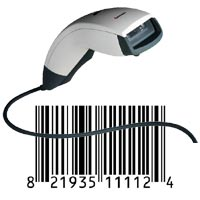
\includegraphics[scale=1.0]{images/Barcodescanner.jpg}
	\caption{Abbildung eines Barcodescanners}
	\label{fig:barcodescanner}
\end{figure}
An einem Zentralen Rechner werden die Bestellungen der Kunden ausgedruckt. Solch ein Ausdruck besteht aus einer Seite, auf der oben zwei Adressetiketten und unten einem Lieferschein vorhanden sind. Das erste Adressetikett ist das f�r den Versand zu dem Kunden, das auf den Umschlag der Bestellung geklebt wird. Das zweite ist dasjenige, welches der Kunde auf dem Umschlag zur R�cksendung der Video klebt. Der Lieferschein ist sowohl f�r den Mitarbeiter als auch f�r den Kunden wichtig. Der Mitarbeiter liest mit Hilfe eines Barcodescanners die Bestellnummer ein. Aus dieser Rechnungsnummer kann der Computer sowohl auf den Kunden als auch auf die Videos schlie�en, die versendet werden sollen. Der Mitarbeiter sucht, mit Hilfe einer weiteren Software den Lagerort der jeweiligen Videos heraus und scannt deren eindeutige Nummer. Damit sind die Videos im System nicht mehr verf�gbar und dem Kunden zugeordnet. Anschlie�end verpackt er die Videos in einen entsprechenden Umschlag und verschickt die Videos mit dem Ausdruck an dem Kunden. Bei diesem Vorgang gibt es mehrere M�glichkeiten wie der Mitarbeiter vorgehen kann. Damit der Mitarbeiter nicht f�r jede Bestellung durch das Lager gehen muss, kann das System eine Liste mit Videos erstellen, f�r die n�chsten 10 Bestellungen. Somit sucht der Mitarbeiter diese Videos heraus und bearbeitet nacheinander diese zehn Bestellungen. Eine weitere M�glichkeit w�re, das der Mitarbeiter und das Lager durch ein automatisiertes Lager ersetzt wird. Dabei �bernimmt ein Roboter in einem Lager die Aufgabe des Suchen und Finden der Videos. Schickt der Kunde die Videos an die Online-Videothek zur�ck, nimmt ein Mitarbeiter die Videos entgegen. Zuerst scannt er dabei die Bestellnummer und die eindeutige Nummer des jeweiligen Videos. Zus�tzlich muss er den Zustand der Videos �berpr�fen und im System eintragen. Anschlie�end sind die Videos wieder im System verf�gbar und k�nnen wieder eingeordnet werden oder an den n�chsten Kunden versendet werden.\\
Das komplette Lager k�nnte durch spezielle Maschinen vollst�ndig automatisiert werden. Diese Maschinen w�rden dann automatisch das Suchen und das Verpacken der Videos �bernehmen. Dabei w�rden wieder Barcodescanner zum Einsatz kommen, um die Bestellnummern und Videonummers automatisch einzulesen. Solch ein System w�rde sich aber nur bei einer sehr grosser Online-Videothek rentieren, da der Anschaffungspreis solcher Maschinen enorm ist.

\begin{figure}[tbp]
	\centering
	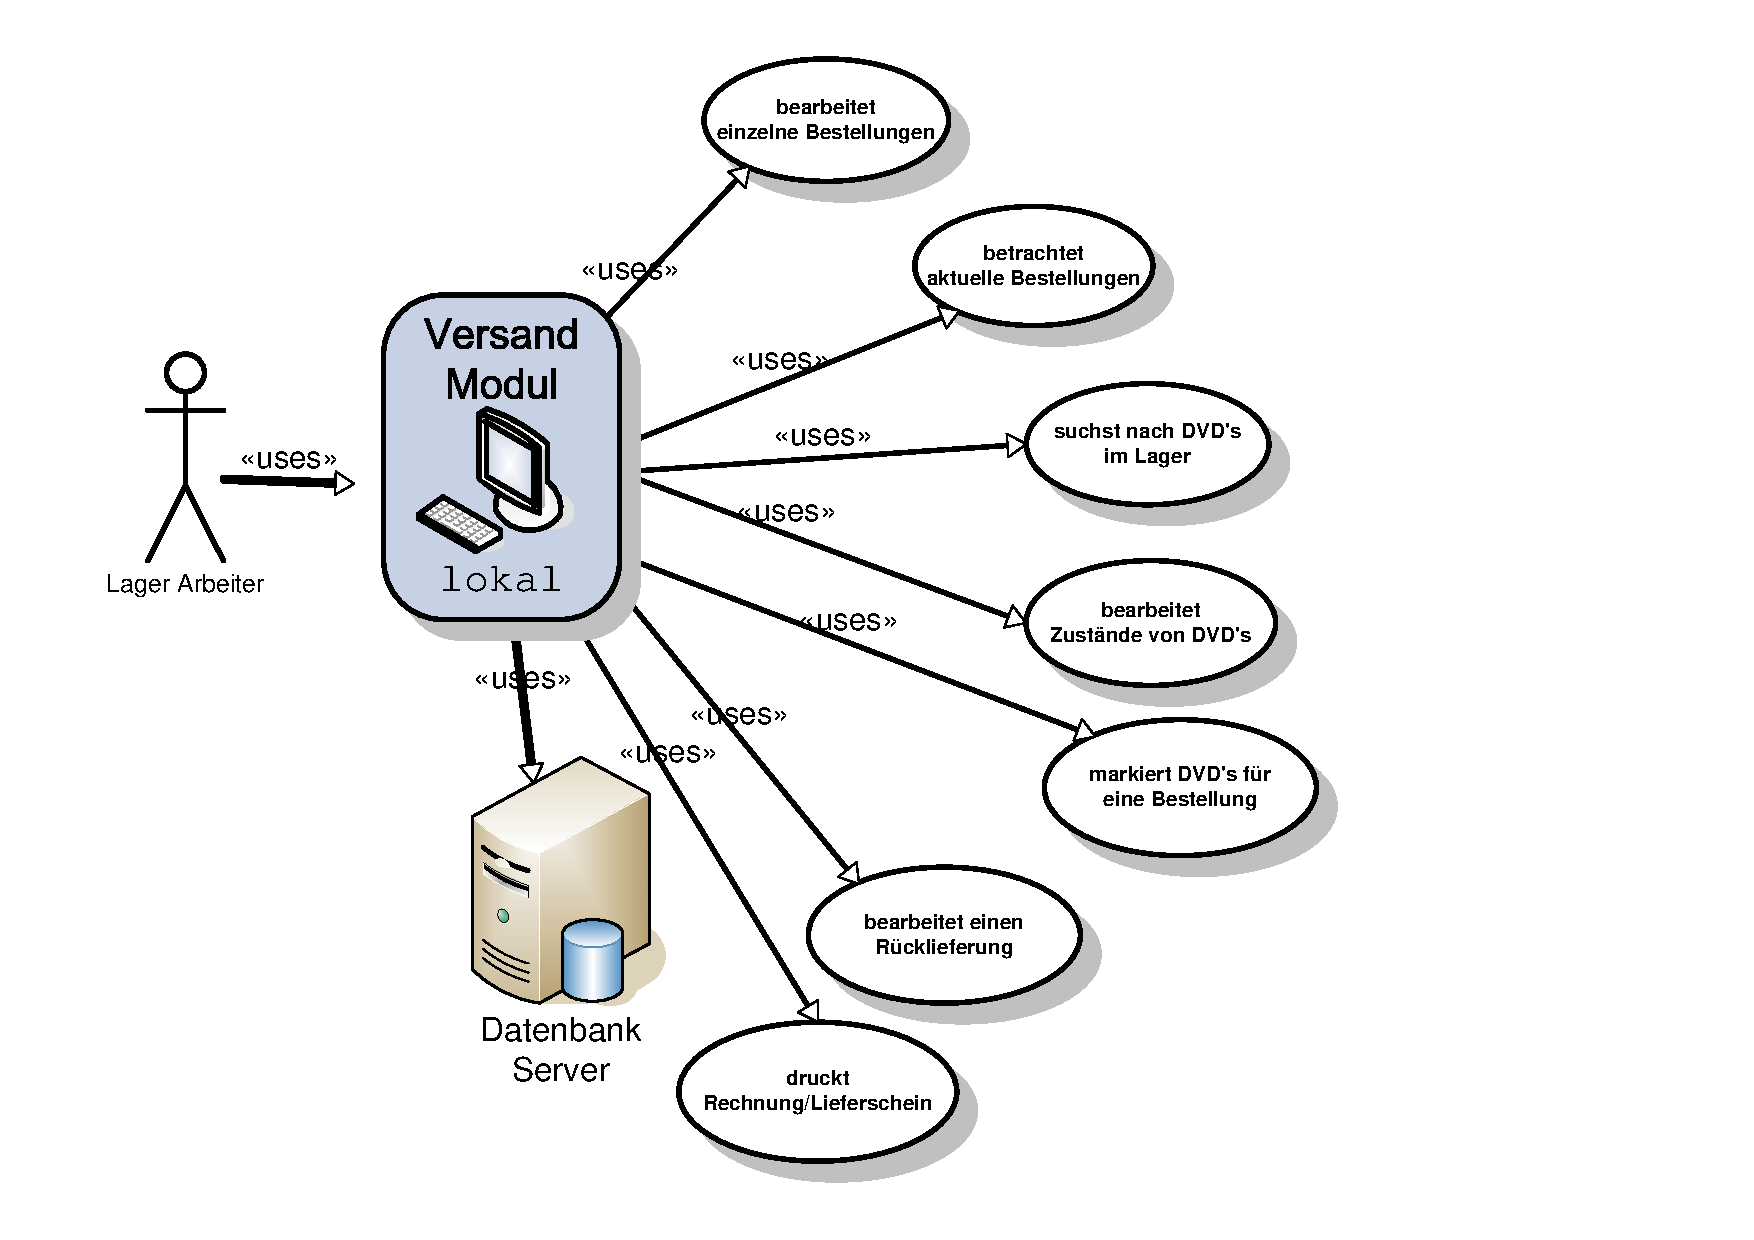
\includegraphics[scale=1.0]{images/usecase-versandmodul.pdf}
	\caption{UseCase Versandmodul}
	\label{fig:usecaseversand}
\end{figure}
	 	
%===========================================
\subsection{das Verwaltungsmodul im Detail}  \label{sec:Verwaltungsmodul}
Das Verwaltungsmodul ist f�r die Verwaltung der Online-Videothek in B�ror�umen gedacht. Die Mitarbeiter des Unternehmens haben dabei Einblick in die verschiedenen Daten der Online-Videothek und k�nnen diese, sollten sie die ben�tigten Rechte besitzen, ver�ndern. Unter zu Hilfenahme des Verwaltungsmodul k�nnen neue Videos in System aufgenommen werden. Dazu wird zuerst der jeweilige Film hinzugef�gt und danach die einzelnen Videos dieses Filmes. Dabei werden sich wiederholende Daten wie Darsteller oder Genre in eigenen Elementen gespeichert. Nachdem der Mitarbeiter mit dem Hinzuf�gen von neuen  Videos fertig ist, werden diese automatisch im Kundenmodul verf�gbar sein. Mit Hilfe dieses Moduls k�nnen auch Kundendaten betrachtet oder ver�ndert werden. Somit kann z.B. eine Telefonhotline oder der Kundensupport Fragen der Kunden zu einzelnen Bestellungen beantworten. F�r die Gesch�ftsleitung k�nnen ausf�hrliche Statistiken erstellt werden.\\
Das Verwaltungsmodul stellt somit ...
\begin{figure}[htbp]
	\centering
	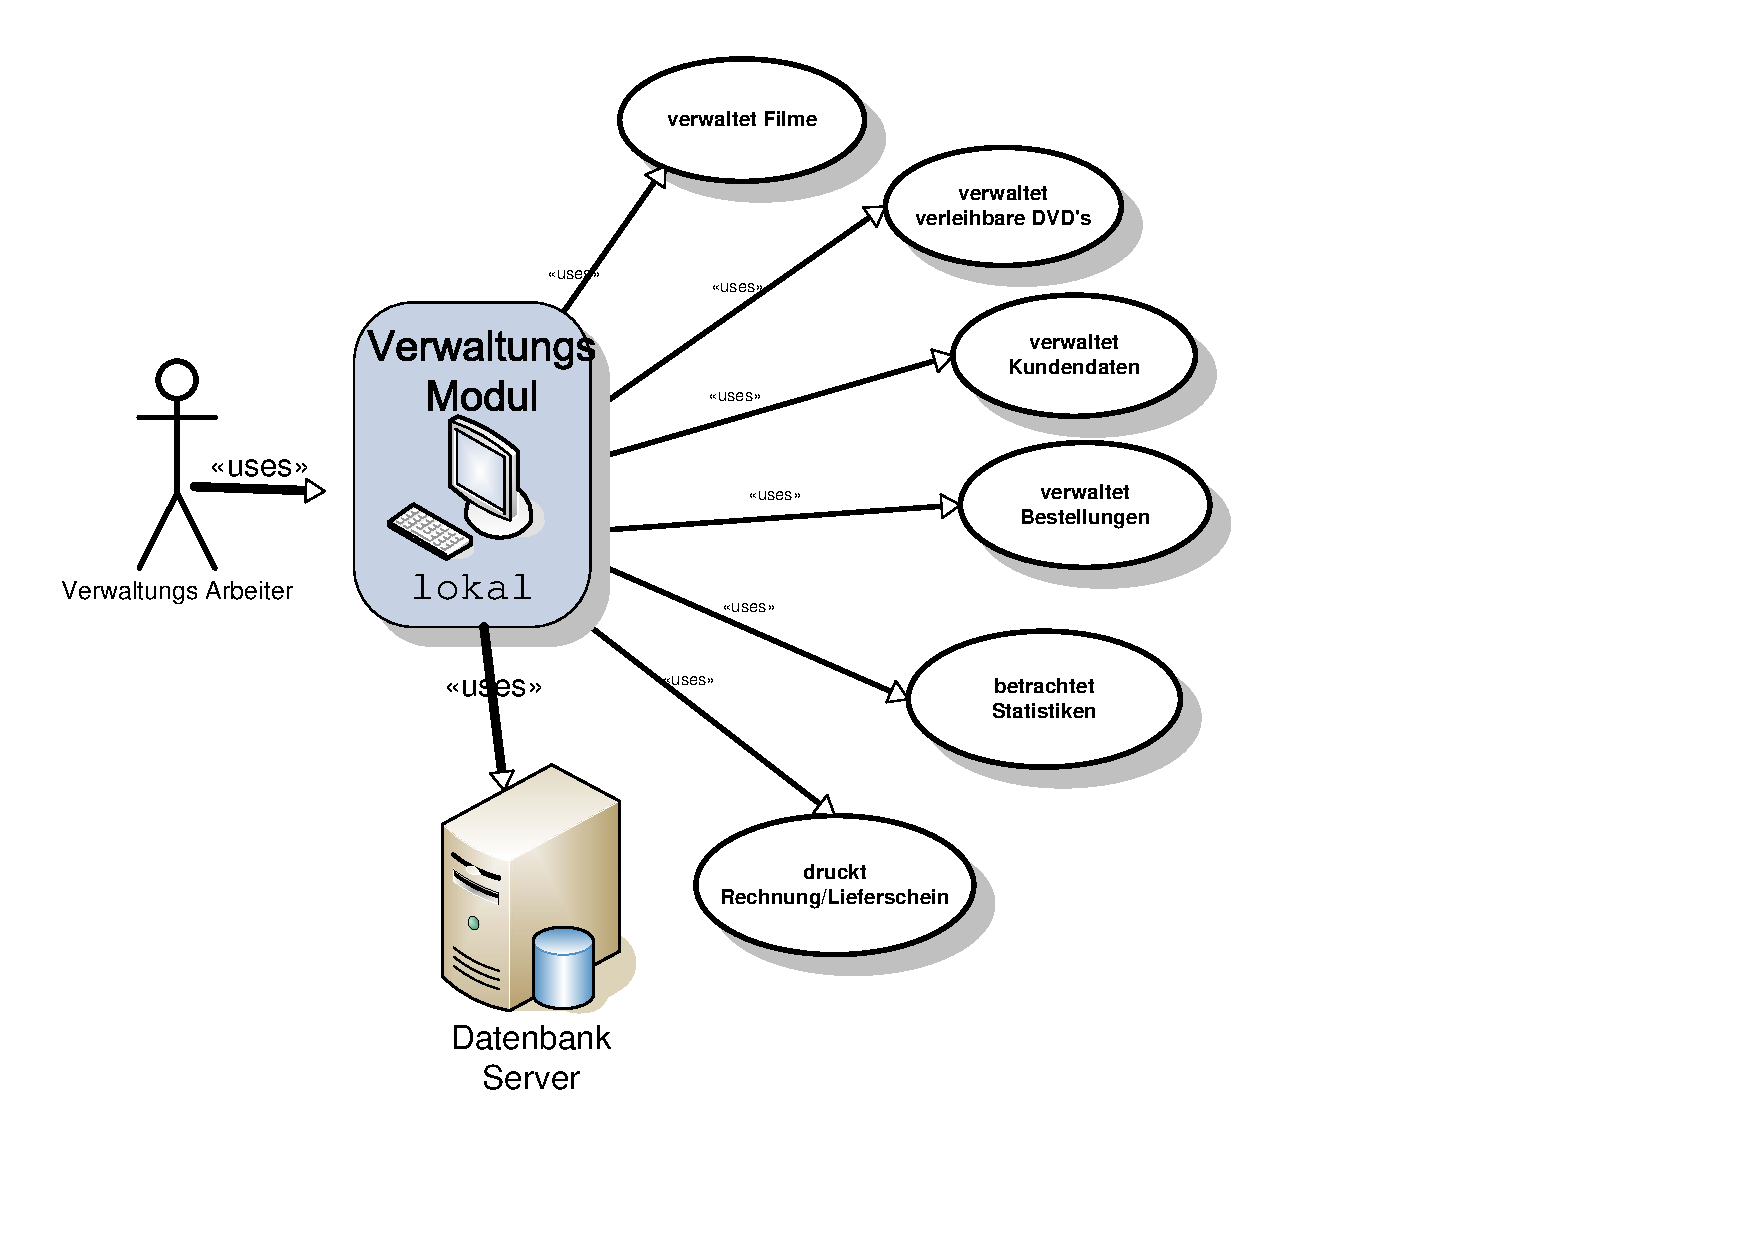
\includegraphics[scale=1.0]{images/usecase-verwaltungsmodul.pdf}
	\caption{UseCase Verwaltungsmodul}
	\label{fig:usecaseverwaltung}
\end{figure}



%===========================================
\section{geplante Module und Versionen}
Da dieses Projekt nach ersten �berlegungen und Planungen nicht nur ein kleiner Projekt ist, wurde beschlossen, zuerst das Verwaltungsmodul, dann das Kundenmodul und danach das Versandmodul zu implementieren. Das Verwaltungsmodul ist das Herzst�ck der Online-Videothek. Hier werden die Daten erstellt und verwaltet, die von den beiden anderen Modulen verwendet werden. Das Verwaltungsmodul und das Versandmodul, soll dabei eine Anwendung auf einem beliebigen Rechner innerhalb des Firmennetzwerks sein. Das Kundenmodul hingegen soll eine weltweit verwendbare Webanwendung sein. Mit der Realisierung des Verwaltungsmodul wurde zuerst begonnen.\\


Das Kundenmodul und das Versandmodul konnten aus Zeitgr�nden nicht mehr realisiert werden.\\


%====================================
\chapter{Technologien} \label{sec:Technologien}
%\section{Datenbank}
Zum Einsatz soll eine OpenSource Datenbank kommen. Gedanken an eine kommerzielle Datenbank kam aus Gr�nden der Lizenzkosten nicht auf. \\
Zu Auswahl standen mehrere OpenSource Datenbanken. MySql \footnote{\url{http://dev.mysql.com/downloads/mysql/4.0.html}}, SAP DB \footnote{\url{http://dev.mysql.com/downloads/maxdb/7.5.00.html}} , HSQL DB \footnote{\url{http://hsqldb.sourceforge.net}} und Firebird \footnote{\url{http://firebird.sourceforge.net}}.
		\begin{itemize}
			\item \textbf{MySql}
				\begin{itemize}
					\renewcommand{\labelitemii}{+}
					\item sehr verbreitet
					\item einige Erfahrung
					\item gut Dokumentiert \& gro�e Community
					\item 
				\end{itemize}
				
				\begin{itemize}
					\item schlechtes Lizenzmodell
					\item zu bekannt
					\item keine Trigger
					\item meist nur im privat bzw. klein Unternehmer Einsatz
				\end{itemize}
				
			\item \textbf{SAP DB}
				\begin{itemize}
					\renewcommand{\labelitemii}{+}				
					\item 
					\item Datenbank seit mehreren Jahren bei SAP im Einsatz
				\end{itemize}
				
				\begin{itemize}
					\item schlechte Skalierbarkeit, da der Datenbank Speicherbereich im Vorfeld festgelegt werden muss
					\item schlechte Erfahrung
				\end{itemize}
				
			\item \textbf{HSQLDB}
				\begin{itemize}
					\renewcommand{\labelitemii}{+}				
					\item reine JavaDatenbank
					\item sehr klein
					\item kann als reine Speicher Datenbank verwendet werden (Daten nur im Arbeitsspeicher)
					\item kann als Applikations Datenbank verwendet werden (nur eine Applikation benutzt die Datenbank)
				\end{itemize}
				
				\begin{itemize}
					\item nicht f�r gro�e Applikationen geeignet
					\item 
				\end{itemize}			

			\item \textbf{Firebird}
				\begin{itemize}
					\renewcommand{\labelitemii}{+}				
					\item geringe Erfahrung durch Studium
					\item sehr klein
					\item gute grafische Tools
					\item Original Sourcen kommen von Borland
					\item Interbase Datenbank seit mehreren Jahren im Professionelle einsatz
				\end{itemize}
				
				\begin{itemize}
					\item schlechtes Lizenzmodell
					\item 
				\end{itemize}
		
		\end{itemize}
		
Wir haben uns f�r die Firebird Datenbank entschieden, da es keine wirkliche Konkurrenz im Open Source Bereich gibt.\\
HSQL scheidet schon aus, weil es nicht f�r grosse Datenmengen geeignet ist. Bei der SAP DB muss der ben�tigte Speicherplatz der Datenbank vorher bekannt sein, was bei unserem Projekt nicht der Fall ist. MYSQL unterst�tzt keine Triggers und ist zu bekannt, d.h. MySql kann und sollte jeder Informatiker kennen und benutzt haben. \\
Firebird ist f�r uns relativ neu und die Erfahrungen die wir in der Vorlesung "`Datenmanagment 2"' bekommen haben, war sehr positiv. Da diese Datenbank urspr�nglich von Borland kommt, ist diese Datenbank auch nicht so neu, wie viele Denken.\\
Es soll aber schon am Anfang des Projektes bedacht werden, dass die Datenbank zu einem sp�teren Zeitpunkt eventuell mit einer professionelle Datenbank\footnote{z.B. DB2 von IBM} ausgetauscht werden k�nnte. Deswegen muss schon am Anfang eine hohe Abstraktionsebene vorhanden sein, so dass eventuelle Datenbankspezifische Elemente (Klassen) sehr einfach ausgetauscht werden k�nnen.
	
\section{Versionsverwaltung} \label{sec:tech-Versionsverwaltung}
Eine Versionsverwaltung 


\url{http://better-scm.berlios.de/comparison/comparison.html}
\citep[Versionsverwaltung]{Wikipedia2005}

\subsection{Concurrent Versions System - CVS}
		
		
\subsection{Subversion}

\begin{figure}[htbp]
	\centering
	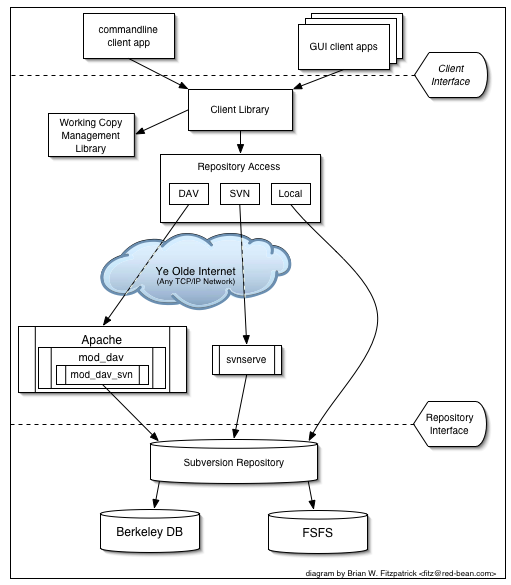
\includegraphics[scale=0.65]{images/subversion-architektur.png}
	\caption{Subversion's Architektur \citep[Kap.~1]{Collins-Sussman2005}}
	\label{fig:svnarchitekur}
\end{figure}


\begin{figure}[htbp]
	\centering
	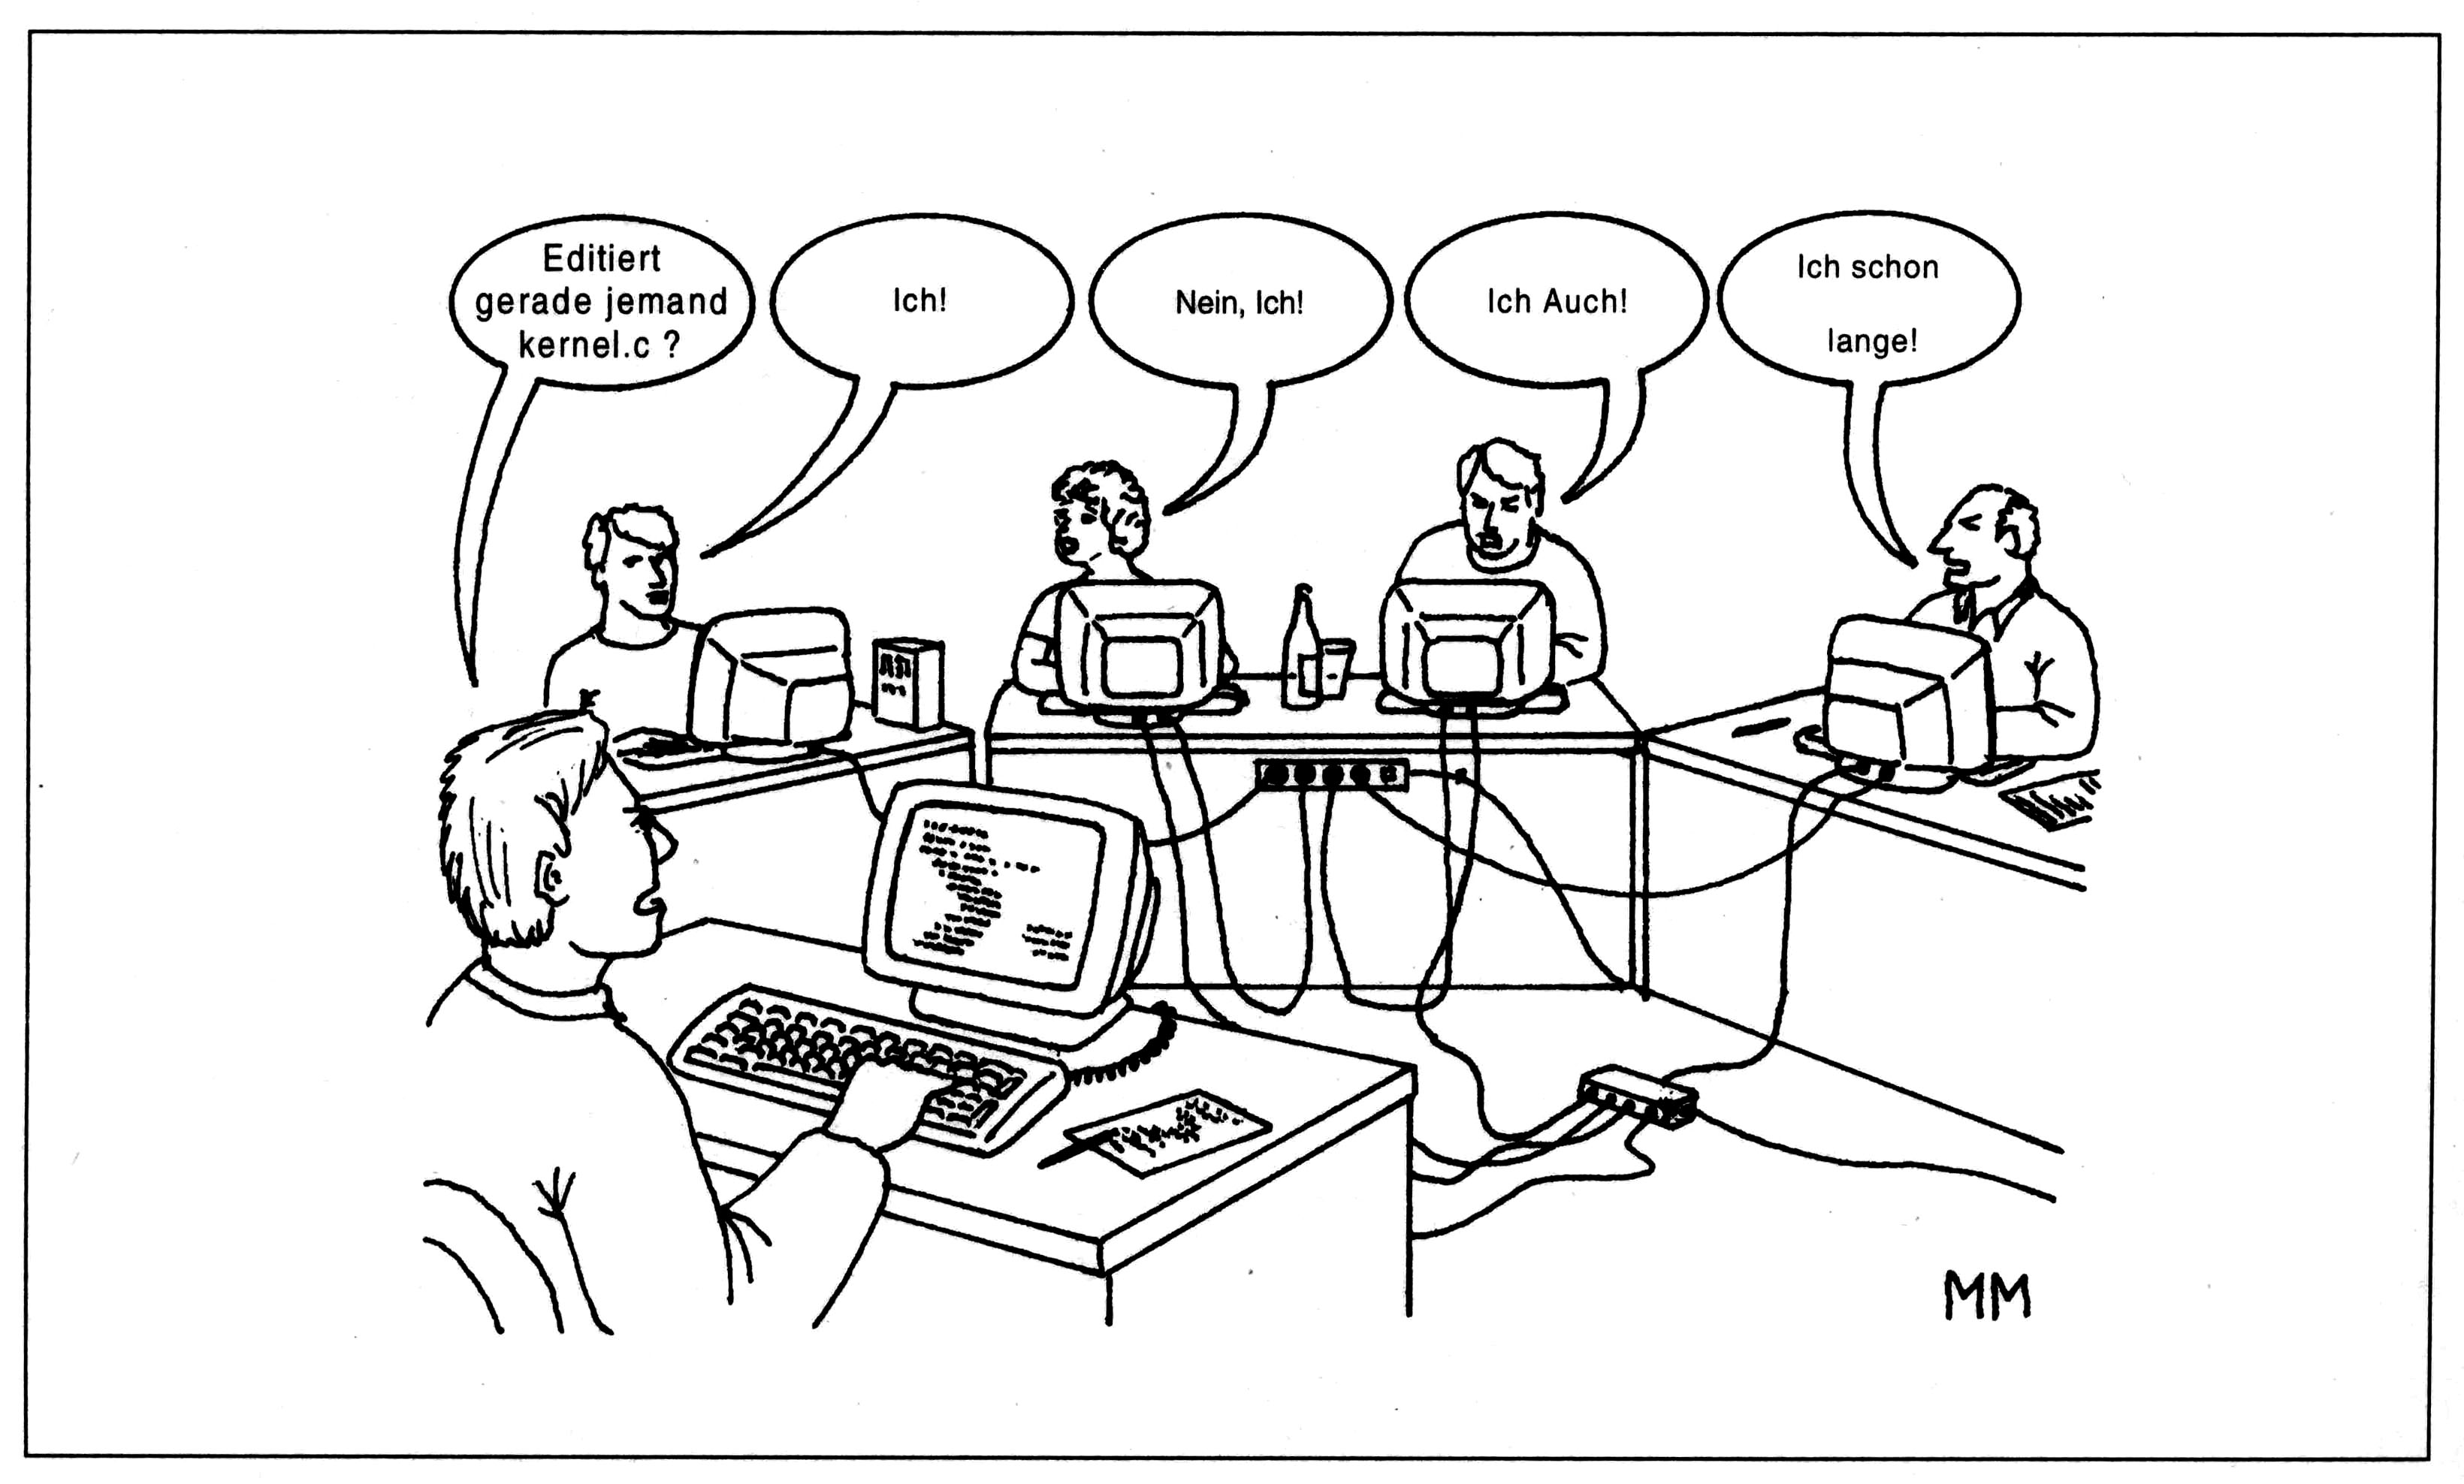
\includegraphics[scale=1.0]{images/vv-personen.jpg}
	\caption{Softwareentwicklungs-Praxis \citep[Bild 2.1]{Herold1995}}
	\label{fig:vv-personen}
\end{figure}



\begin{figure}[htbp]
	\centering
	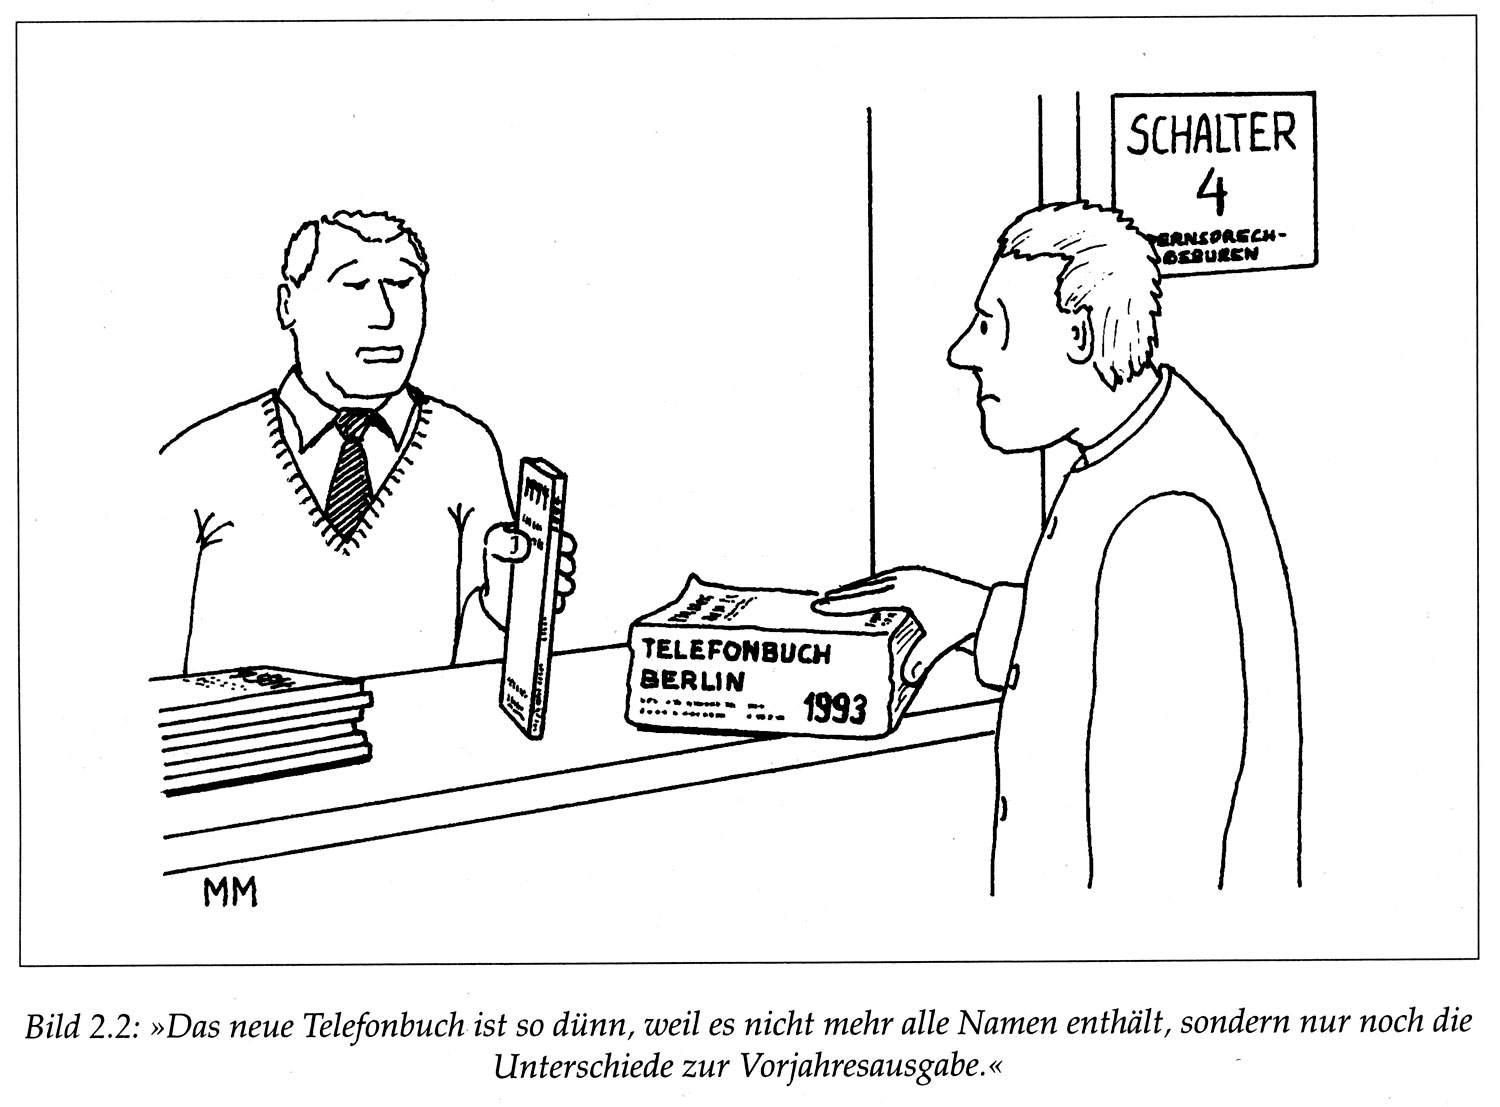
\includegraphics[scale=1.0]{images/vv-speicherbedarf.jpg}
	\caption{Speicherbedarf einer Versionsverwaltung \citep[Bild 2.2]{Herold1995}}
	\label{fig:vv-speicherbedarf}
\end{figure}



%Hier danach nicht mehr schreiben
\label{sec:tech-Versionsverwaltung-ende}
\section{Entwicklungsumgebung} \label{sec:tech-Entwicklungsumgebung}
\subsection{Eclipse}
Eclipse ist eine Open-Source-Framework, das meist als Entwicklungsumgebung genutzt wird und auf 11 verschiedenen Systemen und Architekturen verwendet werden kann. Darunter befinden sich unter anderem Windows, Linux, MAC OS X, etc. Eclipse ist der Nachfolger von Visual Age for Java von IBM. Der Quellcode von Eclipse wurde 2001 von IBM freigegeben. Eclipse bildet nur den Kern, die Funktionalit�t wird �ber Plug-ins realisiert. Je nach verwendeten Plug-ins stellt sich somit die gesamte Funktionalit�t der Entwicklungsumgebung zusammen. Sowohl Eclipse als auch die Plug-ins sind in Java implementiert. Die Plug-Ins sind teilweise frei verwendbar und teilweise kommerziell. Dabei werden neben Java auch andere Sprachen wie zum Beispiel: C, C++. Perl und PHP  unterst�tzt. Das dynamische Hinzuf�gen und Entfernen von Plug-ins und die daraus entstehende Gesamtfunktionalit�t der Eclipse-Entwicklungsumgebung bezeichnet man als Rich Client Platform, das wiederum auf den OSGi-Standard basiert.\\
Der OSGi-Standard (Open Services Gateway Initiative) ist ein Industriekonsortium, das ein  Framework, f�r die Vernetzung von intelligenten Embedded-Ger�ten und das Bereitstellen von Diensten zur Laufzeit erm�glicht, entwickelt hat. Eclipse verwendet das OSGi-Framework au�erhalb dieser Embedded-Ausrichtung.\\
F�r die GUI-Erstellung wurde in Eclipse SWT verwendet, da SWT auf die nativen GUI-Komponenten des jeweiligen Betriebssystems zugreift ist Eclipse, trotz Java, nicht als plattformunbh�ngig zu betrachten.\\
\begin{figure}[htb]
	\centering
	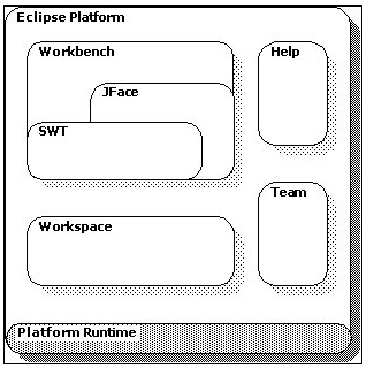
\includegraphics[scale=0.5]{images/Eclipse-Aufbau.png}
	\caption{Aufbau der Eclipse-Plattform}
	\label{fig:eclipse-aufbau}
\end{figure}
Der Aufbau von Eclipse setzt sich dabei aus folgenden Subsystemen zusammen, die teilweise aus einem oder mehreren Plug-ins bestehen wie in \vref{fig:eclipse-aufbau} zu sehen ist.
Die einzelnen Subsysteme definieren Erweiterungs-Schnittstellen um deren Funktionalit�t der Plattform zug�nglich zu machen, wie in Tabelle 3.1 auf Seite \pageref{tab:eclipse-subsystem} zu sehen ist. 

\begin{table}[htbp]
	\centering
	
\begin{longtable}{|c|p{10cm}|}
\caption{Subsysteme von Eclipse}\\

\hline
\textbf{Subsystem} & \textbf{Funktion} \endhead
\hline
Plattform-Runtime & Definiert die Erweiterungs-Schnittstellen und das Plug-in Model. Es findet dynamisch Plug-ins und enth�lt Informationen zu den Plug-ins und deren Schnittstellen in einem Register. Die eingef�gten Plug-ins werden gestartet, wenn der Anwender sie �ber die Plattform aufruft. \\
\hline
Resource Management & Definiert die API f�r das Erzeugen und Verwalten von Projekten, Dateien und Verzeichnissen, die von Tools erzeugt wurden und im Dateisystem abgelegt sind.\\
\hline
Workbench (UI) & Implementiert das Bedienfeld um mit der Plattform zu arbeiten. Definiert Erweiterungs-Schnittstellen f�r weitere UI-Komponenten, um vorhandene Funktionalit�ten aus bereits bestehenden Ansichten und Men�s zu erweitern oder zu verwenden. Als Grundlage dienen dazu JFace und SWT, die im Kapitel SWT beschrieben sind.\\
\hline
Help System & Definiert Erweiterungs-Schnittstellen f�r Plug-ins, um eine Hilfe oder andere Informationen als durchsuchbare B�cher bereitzustellen. \\
\hline
Team Support & Definiert ein Team-Programmierungsmodell zum Verwalten von Ressourcen. \\
\hline
Debug Support & Definiert ein sprachunabh�ngiges Debug-Modell und UI-Klassen f�r das Erstellen von Debuggern und Launchers.\\
\hline
Other Utilities & Andere n�tzliche Plug-ins unterst�tzen Funktionen f�r das Vergleichen von Ressourcen, das Erzeugen von Konfigurationen �ber XML-Files und das dynamische Updaten der Plattform �ber einen Server.\\
\hline
			
\end{longtable}
\label{tab:eclipse-subsystem}
\end{table}





\citep[Eclipse]{Wikipedia2005}
\citep{EclipseISV}



%Hier danach nicht mehr schreiben
\label{sec:tech-Entwicklungsumgebung-ende}
\section{grafische Benutzerschnittstellen in Java} \label{sec:tech-Benutzerschnittstellen}
\subsection{Abstract Window Toolkit - AWT}
Die Abk�rzung AWT steht f�r Abstract Window Toolkit. AWT stellt eine Standard-API f�r die Erzeugung und Darstellung von plattformunabh�ngigen Benutzerschnittstellen f�r grafische Oberfl�chen in Java zur Verf�gung. AWT verwendet die nativen GUI-Komponenten des jeweiligen Betriebssystem zur Darstellung der grafischen Oberfl�chen. Da diese nativen GUI-Komponenten teilweise mit umfangreichen Betriebssystemressourcen verbunden sind, wird AWT auch als Heavyweight-Framework bzw. die einzelnen GUI-Elemenete als Heavyweight-Components bezeichnet.\\ 
Seit dem JDK ( Java Development Kit ) 1.0 steht AWT als Grafik-Bibliothek f�r die Anwender zur Verf�gung. Dabei l�sst sich AWT in 4 Gruppen unterteilen:
\begin{itemize}
	\item Grafische Primitivoperationen zum Zeichnen von Linien oder F�llen von Fl�chen und zur Ausgabe von Text
	\item	Methoden zur Steuerung des Programmablaufs �ber Nachrichten durch Tastatur-, Maus- oder Fensterereignisse.
	\item Portables Design f�r Dialogboxen zur Darstellung der Dialogelemente und die Kommunikation mit dem Anwender
	\item Fortgeschrittene Grafikfunktionen f�r die Bearbeitung und Darstellung von Bitmaps, sowie zur Ausgabe von Sound
\end{itemize}
Aufgrund der hohen Performance-Anspr�che von AWT, besonders f�r gro�e GUI-Anwendungen, wurde es im JDK 1.1 von SUN massiv ver�ndert. Dabei wurden viele Fehler behoben und auch viele Methodennamen ver�ndert. Des Weiteren wurde das Event Handling-Modell, also der Transfer von GUI-Ereignissen, komplett �berarbeitet. Dazu wurde AWT die F�higkeit gegeben GUI-Ereignisse an beliebige Objekte zu �bergeben und dort abzuarbeiten. Aufgrund dieser F�higkeit erreicht man eine klare Trennung zwischen Benutzeroberfl�che und Applikationslogik.\citep{Krueger2003}




\subsection{Swing}
Swing ist eine weitere Grafikbibliothek die im JDK 1.1 als Add-on verf�gbar war und seit Version 1.2 fester Bestandteil des Java Development Kit ist. Swing wurde von SUN entwickelt um die grafische Benutzeroberfl�che von Java Programmen zu verbessern, da man folgende Eigenschaften von AWT als nachteilig ansah:
\begin{itemize}
	\item Aufgrund der Verwendung der jeweiligen nativen GUI-Elemente des eingesetzten Betriebssystems, war es sehr schwer ein einheitliches Look-an-Feel ( Aussehen ) zu realisieren.
	\item Um das Verhalten der verschiedenen GUI-Elemente der einzelnen Betriebssysteme ann�hernd anzugleichen war sehr viel Portierungsaufwand notwendig.
	\item Des Weiteren gibt es in AWT nur eine Grundmenge an Dialogelementen mit denen sich aufwendige grafische Oberfl�chen nur mit sehr viel Zeitaufwand realisieren lassen.
\end{itemize}
Das Ziel der Entwickler war es diese Nachteile mit Swing zu beseitigen.\\
Um einen Teil der Nachteile zu beseitigen, greift Swing nur noch eingeschr�nkt auf die jeweiligen nativen GUI-Elemente zu. Die restlichen GUI-Elemente werden von Swing selbst erzeugt und gezeichnet.
\begin{itemize}
	\item Aufgrund dieser Vorgehensweise f�llt ein Gro�teil der plattformspezifischen Besonderheiten weg.
	\item Des Weiteren entf�llt die unterschiedliche Bedienung und Darstellung zwischen den verschiedenen Betriebssystemen, so dass ein Anwender auf allen Betriebssystemen dasselbe Aussehen vorfindet.
	\item Zus�tzlich ist SWING nicht mehr angewiesen auf den kleinsten gemeinsamen Nenner der GUI-Elemente der Betriebsysteme aufzubauen, sondern kann unabh�ngig davon komplexere GUI-Elemente bereitstellen ohne auf das jeweilige Betriebssystem zu achten. Au�erdem stehen in Swing dem Programmierer viel mehr Dialogelemente zur Verf�gung als das bei AWT der Fall war.
\end{itemize}

\subsubsection{Leichtgewicht-Komponenten}
Die GUI-Elemente in Swing werden als Lightweight-Components bezeichnet, da sie nicht mehr �ber die betriebssystemspezifische Klassen erstellt werden m�ssen, sondern durch Komponenten-Klassen mit Hilfe von Primitivoperationen erzeugt werden.\\
Mit Hilfe der Leichtgewicht-Komponenten war es zus�tzlich m�glich, Tooltips ( kleine Fenster mit n�tzlichen Informationen ) unabh�ngig vom verwendeten Grafiksystem und einem Debug-Modus ( Debug-Grafik ) zum Finden von Fehlern w�hrend der Erzeugung von grafischen Oberfl�chen zu implementieren.


\subsubsection{Pluggable Look-and-Feel}
Eine der spektakul�rsten Eigenschaften von Swing ist das Look-and-Feel der GUI-Elemente zur  Laufzeit zu ver�ndern. Dabei hat der Anwender die M�glichkeit zwischen einer bestimmten Menge an Look-and-Feels auszuw�hlen. Des Weiteren ist es m�glich auch eigene Look-and-Feels zu erstellen.\\
Die Entscheidung, welches Look-and-Feel verwendet werden soll, muss dazu nicht w�hrend der Design-Phase entschieden werden. Man kann dem Anwender ein Men� zur Verf�gung stellen, indem er w�hrend der Laufzeit das ihm passende Look-and-Feel ausw�hlt. Das Umschalten erfolgt praktisch ohne weiteren Aufwand des Programmes, es wird von einem User-Interface-Manager erledigt, der alle notwendigen Ma�nahmen ausf�hrt.


\subsubsection{Das Model-View-Controller Prinzip}
Beim Model-View-Controller Prinzip wird nicht die gesamte Funktionalit�t in eine Klasse gepackt sondern in drei Bestandteile zerlegt:
\begin{itemize}
	\item Das Modell enth�lt die Daten des Dialogelementes und speichert seinen Zustand.
	\item Der View ist f�r die grafische Darstellung der Komponente verantwortlich.
	\item Der Controller wirkt als Verbindungsglied zwischen dem Modell und dem View und st��t bei Ereignissen die notwendigen Ma�nahmen zur Ver�nderung von Modell und View an.
\end{itemize}
Eine wichtige Eigenschaft bei diesem Prinzip ist, dass ein Modell mehrere Views gleichzeitig haben kann. Dazu werden bei Ver�nderungen am Modell die Views benachrichtigt und aktualisieren sich entsprechend.\\
Bei Swing sind der View und der Controller in einer Klasse untergebracht, dadurch wird die Komplexit�t reduziert. Au�erdem ist in den meisten F�llen der Controller so einfach strukturiert, dass es sich gar nicht lohnt ihn in einer zus�tzlichen Klasse zu implementieren.\\
Die hier genannten Eigenschaften bringen aber auch Nachteile mit sich:
\begin{itemize}
	\item Swing-Anwendungen sind ressourcenhungrig. Da alle Komponenten selbst gezeichnet werden m�ssen, erfordert es eine h�here CPU-Leistung und Hauptspeicher.
	\item Im JDK 1.2 gab es Speicherprobleme mit Swing-Elementen, da diese den Speicher, den sie belegten, nicht wieder komplett freigaben und sich dadurch der verf�gbare Speicher mit der Zeit verringerte.
	\item F�r Applet-Programmierer gab es keine Browser mit eingebauter Swing-Unterst�tzung, dies muss dem Anwender durch einen zus�tzlichen Download ( der enstsprechenden Bibliothek ) und Installationsschritt zugemutet werden. Eine andere Alternative w�re auf AWT zur�ckzugreifen.
\end{itemize}
Aufgrund der steigenden Rechenleistung der PCs und der im JDK 1.3 verbesserten Swing-Grafikbibliothek konnten jedoch viele der Probleme behoben werden. \citep{Krueger2003}


\subsection{Standard Widget Toolkit und JFace}\label{sec:StandardWidgetToolkitundJFace}
SWT ist ebenfalls eine Grafikbibliothek f�r Java und steht f�r Standard Widget Toolkit. Im Gegensatz zu den anderen genannten Grafikbibliotheken ist SWT von IBM und nicht von SUN entwickelt wurden. SWT wurde im Jahr 2001 f�r die Entwicklungsumgebung Eclipse entwickelt. Im Gegensatz zu Swing verwendet SWT die nativen grafischen Elemente des Betriebssystems und schlie�t sich damit AWT an.\\
Des Weiteren ist SWT, im Gegensatz zu AWT und Swing, nicht als plattformunabh�ngig zu betrachten. Dies resultiert daraus, dass  SWT die entsprechende Bibliothek f�r den betriebssystemabh�ngigen Code f�r die GUI-Elemente zur Laufzeit ben�tigt. Zus�tzlich werden die  Java-Klassen der SWT-Bibliothek ben�tigt, die auf die betriebsystemabh�ngige Bibliothek zugreifen.\\
Leider leidet SWT aufgrund des eben beschriebenen Sachverhaltes auf einigen nicht Windows-Plattformen an Effizienzproblemen, da bestimmte Funktionalit�ten eventuell nicht verf�gbar sind und dadurch emuliert werden m�ssen. Aufgrund des nicht vorhersagbaren Zeitpunktes an dem nicht mehr verwendete Objekte durch den Garbage Collector freigegeben werden, hat IBM implementiert, dass alle erstellten Objekte selbst freigegeben werden m�ssen. Durch diese Vorgehensweise wird sicher gestellt, dass der komplette Speicher, den ein SWT-Objekt belegt, wieder freigegeben wird. Dies bedeutet f�r einen Programmierer zus�tzlichen Aufwand, da der Programmierer daf�r verantwortlich ist, erzeugte Objekte wieder freizugeben.\\
JFace ist ein UI-Toolkit und setzt aus den gelieferten Basiskomponenten von SWT komplexere Widgets zusammen. JFace kann daher �berall eingesetzt werden, wo auch SWT zur Verf�gung steht.\citep[SWT]{Wikipedia2005} \citep{SWTBasic}
		
Krueger2003
SWTBasic
EclipseISV
		






















%Hier danach nicht mehr schreiben
\label{sec:tech-Benutzerschnittstellen-ende}
\section{Java-Web-Anwendungen} \label{sec:tech-WebAnwendungen}
		
%%%%%%%%%%%%%%%%%%%%%%%%%%%%%%
%      Kapitel JSF           %
%%%%%%%%%%%%%%%%%%%%%%%%%%%%%%		
\subsection{Java Server Faces - JSF}
		
Nach \citep{Bill2004} ist JavaServer Faces (JSF) ein komponenten-abh�ngiges Web-Framework, mit dessen Hilfe sich Benutzerschnittstellen mit einer Reihe von wiederverwendbaren GUI-Komponenten, z.B. Labels, Buttons, Eingabefelder usw.,einfach erstellen lassen. JSF ist ein erster offizieller Standard von Sun hinsichtlich der Erstellung von UIs\footnote{User Interface (engl. Benutzerschnittstelle)} von Webanwendungen und wurde im Rahmen des Java Community Process (JCP) unter dem JSR 127\footnote{\url{http://www.jcp.org/en/jsr/detail?id=127}} im September 2002 ver�ffentlicht. Im Experten-Gremium sind viele namhafte Firmen wie IBM, BEA, IONA, Novell, Borland, HP, Oracle oder Siemens, wodurch eine gro�e Unterst�tzung seitens der Industrie erwartet wird.

\begin{figure}[h]
	\centering
	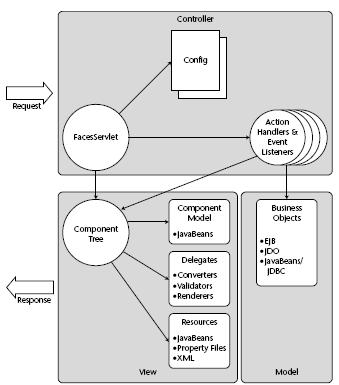
\includegraphics[scale=1]{images/Architektur-JSF.jpg}
	\caption{Architektur von JSF \citep[Bild 1.6]{Bill2004}}
	\label{fig:architecture_jsf}
\end{figure}

Die auf dem bekannten Model View Controller 2(MVC2)-Modell basierende JSF-Technologie besteht aus den folgenden zwei Hauptkomponenten:

\begin{itemize}
	\item JSF API
	\item JSF Tag Libraries
\end{itemize}

Das Pr�sentations-Framework JSF muss die von MVC definierten Komponenten abbilden. Wie in \vref{fig:architecture_jsf} zu sehen ist, wird das Modell durch einfache JavaBeans, aber auch durch EJBs\footnote{Enterprise Java Beans} oder JDOs\footnote{Java Data Objects} abgebildet. Der Controller wird durch Action Handler bzw. Event Listener der jeweiligen UI-Komponenten dargestellt. Im Zentrum des Controllers steht das FacesServlet, welches mit Hilfe der Konfiguration reagieren, agieren und navigieren kann. JSPs und Komponenten sowie deren Renderer, Converter und Validatoren bilden die Views ab. In jeder View, welche meistens durch eine JavaServer Page (JSP) aufgebaut ist, existiert ein entsprechender Component Tree. Dieser beinhaltet alle Komponenten, die in der JSP durch definierte Tags dargestellt werden. Somit hat der Entwickler Zugriff auf alle Komponenten im Laufe des Lebenszyklus der Request-Bearbeitung.

Dieser Lebenszyklus wird zu jeder Anfrage an die JSF-Applikation durchlaufen und enth�lt folgende Phasen:
 
\begin{enumerate}
	\item Restore View: Aufbau des Component Tree
	\item Apply Request Values: Die Daten aus dem Request werden den Komponenten zugeordnet
	\item Process Validations: Die Variablen der Komponenten werden validiert
	\item Update Model Values: Die Variablen der Komponenten werden in deren Datenmodellen gespeichert
	\item Invoke Application: Ausf�hrung der Business-Logik
	\item Render Response: Der Component Tree wird aktualisiert und ein Response generiert
\end{enumerate}		

Die Navigation in einer JSF-Applikation wird in einer Konfigurationsdatei definiert. Darin ist f�r jede JSP jeweils eine Navigationsregel festgelegt. Diese Regeln bestehen aus der Aufrufenden Seite sowie verschiedenen Navigationsf�llen. Solche Fallunterscheidungen machen die Navigation abh�ngig von den Ergebnissen der Businesslogik und sorgen f�r die Dynamik der Anwendung. (vgl. \citep[S.~46ff]{Oeztuerk2004})\\

\textbf{Fazit:} Da in der Projektplanungsphase die derzeitige JSF-Spezifikation zwar relativ ausgereift war, aber noch nicht in einer Finalversion vorlag, wurde in der Phase der Implementierung auf dessen Verwendung verzichtet und stattdessen auf Apache Struts zur�ckgegriffen.

\newpage

%%%%%%%%%%%%%%%%%%%%%%%%%%%%%%
%      Kapitel Struts        %
%%%%%%%%%%%%%%%%%%%%%%%%%%%%%%
\subsection{Apache Struts}

Struts basiert auf dem Model 2 (MVC 2) und ist ein leistungsstarkes und frei erh�ltliches Framework. Hierbei wird die Pr�sentationsebene durch JavaServer Pages konstruiert, der Model-Teil durch JavaBeans �bernommen und Servlets als Controller dieses Frameworks eingesetzt.
Das Struts Framework Projekt wurde nach \citep{ASF2005} im Mai 2000 von Craig R. McCalahan ins Leben gerufen und versuchte die Vorteile von Java Servlets und JavaServer Pages zu vereinen. Zu Beginn wurde ein Model-View-Controller Framework f�r die Java-Welt erarbeitet, welches im Juli 2001 von der Apache Software Foundation (ASF) unter dem Namen Struts 1.0 ver�ffentlicht wurde.  Die ASF ist eine ehrenamtlich arbeitende Organisation zur F�rderung der Apache-Softwareprojekte. Sie entstand im Juni 1999 aus der Apache Group und soll den Apache Open-Source-Software Projekten organisatorische, juristische und finan-zielle Unterst�tzung zur Verf�gung stellen. Die ASF ist eine nicht kommerzielle Organisation aus Entwicklern, die an Open-Source-Softwareprojekten arbeiten. Auch Struts ist ein Open-Source Projekt und unterliegt der Apache Software License\footnote{\url{http://www.apache.org/licenses/}}.

\begin{figure}[h]
	\centering
	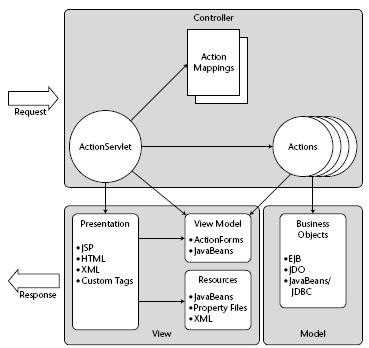
\includegraphics[scale=1]{images/Architektur-Struts.jpg}
	\caption{Architektur von Struts \citep[Bild 1.5]{Bill2004}}
	\label{fig:architecture_struts}
\end{figure}

\newpage

Wie bereits erw�hnt, verfolgt Struts das Model2-Konzept und l�sst sich somit in die drei Komponenten (Model, View und Controller) unterteilen. \vref{fig:architecture_struts} gibt einen �berblick der Architektur von Struts, welche diese Komponenten vereint. Diese einzelnen Komponenten werden in den folgenden Abschnitten detailliert beschrieben.

\subsubsection*{Die Strutskomponente Model}

Das Model von Struts wird durch JavaBeans implementiert. Je nach Funktionalit�t
k�nnen sie in drei Kategorien unterteilt werden:

\begin{itemize}
	\item Beans f�r den Systemzustand
	\item Beans f�r die Anwendungslogik
	\item ActionForm-Beans
\end{itemize}

Die Beans f�r den Systemzustand repr�sentieren die Zustandsinformationen des Systems �ber
deren Attribute. Der interne Zustand der Anwendung wird somit durch eine oder mehrere Beans und den Attributen dargestellt. Im Beispiel der Provirent-Anwendung l�sst sich der Einkaufskorb durch ein Bean darstellen, da es beinhaltet, was ein Kunde f�r seine Bestellung ausgew�hlt hat. Zur Darstellung des aktuellen Zustands k�nnen die zugeh�rigen "`get"'- und "`set"'-Methoden aufgerufen werden. Zum Beispiel kann die Anzahl der ausgew�hlten Artikel, die durch das Attribut anzahlArtikel dargestellt wird, �ber den Aufruf der Methode getArtikelAnzahl() abgefragt werden.

Die Anwendungslogik kann durch JavaBeans erg�nzt werden. Damit eine Wiederverwendung der Anwendungslogik gew�hrleistet werden kann, sollten die JavaBeans m�glichst so implementiert werden, dass sie unabh�ngig von der Umgebung der Anwendung ausgef�hrt werden k�nnen. Zum Beispiel sollte die Logik zum Speichern von Bestellungen in die Datenbank ausgelagert werden. Hierbei m�ssen die Funktionalit�ten f�r den Zugriff auf die Datenbank korrekt implementiert werden. Diese Methoden der JavaBeans k�nnen dann sowohl in der Struts-Applikation als auch in anderen Umgebungen, wo Datenbankzugriffe gebraucht werden, aufgerufen werden.

Die ActionForm-Beans dienen zur Behandlung eines Formulars einer Webanwendung. F�r jedes Eingabeformular ist ein entsprechendes ActionForm-Bean vorgesehen. Dieses erm�glicht das Zwischenspeichern von Formulareingabedaten, wobei jedes Eingabefeld einem Attribut der Bean entspricht. Mit der Verwendung von ActionForm Beans ist es m�glich, auf die Daten des Formulars in verschiedenen Bereichen der Anwendung zuzugreifen. Eine solche Bean ist von der Klasse \textit{ActionForm} abgeleitet und kann neben den "`get"'- und "`set"'-Methoden optional noch zwei spezielle Methoden besitzen: \textit{validate}() und \textit{reset}(). Die Methode validate() dient dazu, Eingabedaten aus dem Formular zu validieren. Die Attribute eines Formulars lassen sich durch die Methode reset() zur�cksetzen. Aufgrund der zwingend erforderlichen Namensgleichheit zwischen den Formularelementen und den Attributen der ActionForm Beans wird die Kommunikation zwischen dem Bean und dem HTML-Formular sichergestellt.

\subsubsection*{Die Strutskomponente View}

Die View ist f�r die Pr�sentation der Daten zust�ndig, die meist durch JavaServer Pages umgesetzt wird. Die JSPs k�nnen neben HTML, XML und JavaScript, auch zur Laufzeit dynamisch generierten Code enthalten. Da es m�glichst vermieden werden sollte, Java-Code in die JSP einzubauen werden so genannte Tags eingesetzt. Die JSP-eigenen Tags werden durch die umfangreichen Struts Tag-Bibliotheken (Taglibs) erweitert, wodurch eine gr��ere Funktionalit�t erreicht werden kann. Wie in \vref{code:integration_struts_taglibs} zu erkennen ist, wird jeder einzelnen Bibliothek ein Pr�fix zugeordnet, damit der Compiler diese auseinander halten kann.

\begin{lstlisting}[language=XML, caption={Integration der StrutsTaglibs}, label=code:integration_struts_taglibs, showstringspaces=false]
<\%@ taglib uri="http://struts.apache.org/tags-bean" prefix="bean" \%>
<\%@ taglib uri="http://struts.apache.org/tags-html" prefix="html" \%>
<\%@ taglib uri="http://struts.apache.org/tags-logic" prefix="logic" \%>
<\%@ taglib uri="http://struts.apache.org/tags-tiles" prefix="tiles" \%>
\end{lstlisting}

Neben diesen Bibliotheken lassen sich auch noch eine Reihe anderer Tag-Bibliotheken, wie die Java Standard Tag Library (JSTL), integrieren. Wenn die Funktionalit�ten dann immer noch nicht ausreichen sollten, besteht auch die M�glichkeit, eigene Bibliotheken zu erstellen und zu benutzen. Mit der Verwendung solcher Taglibs wird nach \citep{Cavaness2004} f�r eine deutliche Senkung der Entwicklungszeit und die daraus resultierende Steigerung der Produktivit�t erreicht. Auch die Fehlerbehandlung und die Kommunikation mit den ActionForm Beans wird dadurch vereinfacht. 

Dar�ber hinaus ist man in der Lage, die Web-Anwendung in mehreren Sprachen zu unterst�tzen. Dabei muss die JSP nicht in mehreren Sprachen auf dem Server hinterlegen werden, sondern es k�nnen hierf�r die vom Struts-Framework bereitgestellten Message-Tags verwendet werden. 

\begin{lstlisting}[language=XML, caption={Struts Message-Tag}, label=code:message_tag, showstringspaces=false]
<title>
  <bean:message key="provirent.title"/>
</title>
\end{lstlisting}

An dem Pr�fix \textit{bean} in \vref{code:message_tag} ist zu erkennen, dass dieses Tag der \textit{struts-bean.tld} Bibliothek angeh�rt. Das Attribut \textit{key} verweist auf ein Element einer zentral definierten Datei, in der alle Texte einer Sprache enthalten sind. Es handelt sich hierbei um eine Properties-Datei mit Key-Value Paaren, die f�r jede der unterst�tzten Sprachen vorliegt. Die Schl�ssel werden in den Message-Tags angegeben und verweisen auf die entsprechenden Texte (Values) der jeweiligen Sprache, die in jeder dieser Properties-Dateien enthalten sind. Dies hat den Vorteil, dass keine Texte mehr in den Quellcode der JSP geschrieben werden m�ssen, sondern durch den Einsatz der Message-Tags in der gew�nschten Sprache zu Laufzeit eingef�gt werden. Der Name und der Pfad der Properties-Datei sind frei w�hlbar, m�ssen aber in der Konfigurationsdatei des Frameworks definiert werden. Es muss darauf geachtet werden, dass eine sprachenabh�ngige Properties-Datei der Namenskonvention entspricht, d.h. im Format \verb|<name_der_Message_Datei>_xx.properties|, wobei das \textit{xx} f�r den zweistelligen Code der jeweiligen L�nder bzw. Sprachen steht (z.B. \textit{en} f�r Englisch, d\textit{e} f�r Deutsch). 

F�r die Interaktion von JSPs mit den ActionForm Beans wurden die Standard HTML-Tags in den Struts Taglibs um gewisse Funktionalit�ten erweitert. Prinzipiell kommen alle wichtigen HTML-Elemente  darin vor. Zum Beispiel l�sst sich mit Hilfe des Tags \verb|<html:form\>| ein HTML-Formular erstellen. �ber das Pflichtattribut \textit{action} wird angegeben, wie nach dem Absenden der Formulardaten damit verfahren werden soll. Hierbei kann eine URL angegeben werden. Es ist aber g�ngiger, keine Web-Ressourcen, sondern eine Action-Klasse aufzurufen, was durch die Endung \textit{*.do} gekennzeichnet wird und dem Controller mitteilt, in der struts-config.xml nach dem entsprechenden Pfad zu suchen. Ein solcher Pfad stellt die Verkn�pfung von ActionForm Beans und Action Klassen der JSP dar. Anhand dieser Zuordnungen k�nnen die Formulardaten der ActionForm Bean zugewiesen und validiert werden.

Wenn durch die \textit{validate}()-Methode ein Fehler festgestellt wird, kann dem Benutzer eine entsprechende Fehlermeldung �ber den Tag \verb|<html:errors\>| mitgeteilt werden. Dieser Tag wird nur aktiv, wenn die mit dem Attribut property definierte Fehlermeldung w�hrend der Validierung erzeugt wurde.

Zus�tzlich zu den oben genannten Tags der Struts-Taglibs stehen dem Struts-Framework noch eine Reihe weiterer Tags zur Verf�gung. Es k�nnen auch die Taglibraries der JSTL Spezifikation\footnote{\url{http://java.sun.com/products/jsp/jstl/index.jsp}} eingesetzt werden.


\subsubsection*{Die Strutskomponente Controller}

Der gesamte Ablauf einer Struts-Anwendung wird �ber den zentral im Struts-Framework vorliegenden Controller gesteuert. Dessen Aufgabe ist es, HTTP-Requests vom Client zu empfangen, diese auszuwerten und zu entscheiden, welche Ma�nahme als n�chstes durchgef�hrt werden soll. Wenn z.B. kein Verarbeitungsschritt mehr notwendig sein sollte, so wird die Anfrage direkt an die JSP weitergeleitet, ansonsten an die spezifische Action-Klasse. Besonders vorteilhaft ist nach \citep{Cavaness2004} die an einem zentralen Punkt liegende Ablaufsteuerung der Anwendung durch den Controller. Bei daran notwendigen �nderungen muss nicht die ganze Anwendung sondern nur ein relativ kleiner Bereich des Programms angepasst werden.
Der Controller umfasst folgende Komponenten:

\begin{itemize}
	\item die Klasse ActionServlet
	\item die Datei struts-config.xml
	\item die Klasse ActionMapping
	\item verschiedene Klassen, die sich von der Klasse Action ableiten
\end{itemize}

Jede Anwendung enth�lt genau ein ActionServlet, das alle Requests des Benutzers verarbeitet. Dieses Servlet sucht in der Struts-Konfigurationsdatei nach der Action f�r den gerade zu bearbeitenden Request. Dar�ber hinaus erzeugt und verwendet es ActionForm Beans f�r das Speichern und Validieren von Daten aus HTML-Formularen und ActionForward Klassen f�r die Fortsetzung des Programmflusses. Das Servlet wird von der Klasse \textit{org.apache.struts.action.ActionServlet} abgeleitet und wird in der Konfigurationsdatei \textit{web.xml} registriert.

Bei einem Request an die Web-Applikation, dessen URL mit *.do endet, schaltet sich das Struts-Framework ein, indem das ActionServlet die Anfrage an die in der URL angegebene Action weiterleitet. Dies geschieht �ber ActionMappings, welche in der \textit{struts-config.xml} angegeben sind. 

Ein solches Mapping wird f�r das Abbilden von speziellen Ereignissen auf die zust�ndigen Action-Klassen ben�tigt, was in Struts durch Eintr�ge in die XML-Datei realisiert wird. Der Ablauf der Anwendung kann somit sehr einfach ver�ndert werden, da lediglich eine Datei angepasst werden muss. Dadurch wird die Datei struts-config.xml zum tats�chlichen Mittelpunkt des Frameworks. Ein weiterer Vorteil der Zentralisierung der ActionMappings liegt darin, dass der Ablauf einer Applikation besser zu verstehen ist, wenn dieser nicht im Quellcode versteckt ist. In \vref{code:struts_config_auszug} wird eine solche Konfiguration dargestellt.

\begin{lstlisting}[language=XML, caption={Auszug aus struts-config.xml}, label=code:struts_config_auszug, showstringspaces=false]
<struts-config>

  <form-beans>

    <form-bean name="LoginForm" 
    	type="de.hsharz.provirent.customer.form.LoginForm"/>

  </form-beans>

  <global-forwards>

    <forward name="index" path="/index.do"/>
    <forward name="login" path="/Login.do"/>
    <forward name="logout" path="/Logout.do" />

  </global-forwards>

  <action-mappings>

    <action path="/index" forward="provirent.index"/>
		
    <action path="/Login" input="vkb.scharf.admin.login" 
    	type="de.hsharz.provirent.customer.action.LoginAction" name="LoginForm" 
    	validate="true"/>

  </action-mappings>

  <message-resources parameter="MessageResources"/>

</struts-config>
\end{lstlisting}

Im Bereich \verb|<form-beans>| wird die Zuordnung der HTML-Formulare zu den entsprechenden ActionForm Beans vorgenommen. �ber das Attribut \textit{name} wird dem ActionForm eine Bezeichnung gegeben, unter der es aufgerufen bzw. initialisiert werden kann, w�hrend \textit{type} den vollst�ndigen Namen der zugeh�rigen Java-Klasse angibt.

Der Abschnitt \verb|<global-forwards>| ist dazu notwendig, logische Namen bestimmten URLs (JSPs oder Actions) zuzuordnen. Der Entwickler hat dann die M�glichkeit, im Quellcode diese Namen mit dem Vorteil anzusprechen, dass �nderungen an den URLs nur noch in der Konfigurationsdatei vorgenommen werden m�ssen.

Mit \verb|<action-mappings>| wird die Zuordnung bestimmter Request-URLs auf die Action-Klassen definiert. Dabei wird f�r jedes Ereignis ein eigenes \verb|<action>| Element angelegt. Dessen Attribut \textit{path} gibt die URL der Action an. Nach \vref{code:struts_config_auszug} wird z.B. durch den Aufruf der URL http://localhost:8080/customer/Login.do das ActionMapping \textit{/login} aufgerufen. �ber das Attribut \textit{type} wird der vollst�ndige Pfad der Action-Klasse angegeben, w�hrend \textit{name} den Namen der zugeordneten ActionForm Bean festlegt. Ein weiteres Attribut \textit{input} gibt die URL einer JSP oder Action an, die f�r die Ausl�sung des ActionEvents verantwortlich ist.

Mit dem Element \verb|<forward>| definiert man, �hnlich wie bei den Global Forwards, eine m�gliche URL, die nach dem Ausf�hren der Action-Klasse aufgerufen werden kann. Ein solcher Forward wird einer bestimmten Action zugeordnet, somit kann sie auch nur aus dieser Action-Klasse aufgerufen werden. Der Vorteil der ActionMappings ist, dass man jede beliebige Action-Klasse aufrufen und an jede JSP oder andere Action weiterleiten kann. 

Action-Klassen sind die Schnittstellen zwischen den Benutzeranfragen und der Gesch�ftslogik. Bei deren Erstellung spielen nach \citep{Goodwill2004} folgende Faktoren eine Rolle:

\begin{itemize}
	\item Sie wird von der Klasse \textit{org.apache.struts.action.Action} abgeleitet.
	\item Sie implementiert die \textit{execute}()-Methode und enth�lt die spezifische Logik.
	\item Die neue Action muus kompiliert werden und sich danach in dem Verzeichnis der Web-Applikation befinden ( meistens \textit{/WEB-INF/classes} ).
	\item Es muss ein neues \verb|<action>| Element in der Konfiguration erstellt werden, dass die neue Action abbildet.
\end{itemize}

Die \textit{execute}()-Methode einer Action-Klasse wird aufgerufen, sobald diese die Kontrolle erhalten hat. Nach \citep{Goodwill2004} wird daraufhin die benutzerdefinierte Gesch�ftslogik ausgef�hrt und die Anfrage weitergereicht. Innerhalb dieser Methode werden alle Operationen, die zum Durchf�hren des Requests n�tig sind, durchgef�hrt. Nach \citep{Wolff2004} und \citep{Robinson2004} sind das haupts�chlich:

\begin{itemize}
	\item Authentifizierung des Userstatus (Zugriff auf die Session)
	\item Validierung der Formulareingaben
	\item Zugriff auf die Gesch�ftslogik
	\item Aufbereitung der Ergebnisse aus der Gesch�ftslogik, so dass diese angezeigt wer-den k�nnen, und Aktualisieren der ActionForm
	\item R�ckgabe eines ActionForward-Objektes, das die nachfolgende Aktion angibt
\end{itemize}

Bei der Erstellung von Action-Klassen muss darauf geachtet werden, dass diese thread-safe und reentrant (wiedereintrittsf�hig) sind. Sie sollten also in einer Multi-Thread Umgebung richtig arbeiten k�nnen. Aus diesem Grund sollten nur lokale Variablen und Methoden zum Einsatz kommen. Dar�ber hinaus kann es zu Skalierungsproblemen kommen, wenn f�r jeden Benutzer Ressourcen, wie z.B. Datenbank-Verbindungen, erzeugt und verwendet werden. Solche Ressourcen sollten �ber Pools vergeben werden. 

















%Hier danach nicht mehr schreiben
\label{sec:tech-WebAnwendungen-ende}
\section{Hibernate} 	\label{sec:tech-hibernate}
		
Hibernate ist ein Open Source-Persistenz-Tool, das basierend auf so genannten Mappings das Bindeglied zwischen JavaBeans und einer Datenbank darstellt. Seit September 2003 geh�rt das Hibernate-Projekt zur JBoss Group und liegt in der aktuellen Version 3.0 kostenlos zum Download\footnote{\url{http://www.hibernate.org}} bereit. Zur Zeit werden 16 Datenbanken unterst�tzt, worunter unter anderem Oracle, DB2, MySQL sowie PostgreSQL z�hlen. Zu den weiteren Besonderheiten z�hlen die Hibernate Query Language, Native SQL Queries sowie Lazy- und Outer-Join Fetching zur Steigerung der Performance. Ferner l�sst sich Hibernate problemlos in alle bekannten J2EE Application Server integrieren.\\
Hibernate stellt den Entwicklern ein umfangreiches Werkzeug f�r die Realisierung einer leistungsf�higen Persistenzschicht zur Verf�gung. Hierbei werden grundlegende Mechanismen f�r das Laden, Speichern, Aktualisieren und L�schen von Java-Objekten, sowie deren Beziehungen, bereitgestellt.\\
Das Abbilden von Java-Objekten auf eine entsprechende Datenbank erfolgt auf einem �u�erst flexiblen Weg, da sich diese Java-Klassen und die entsprechenden Konfigurationsdateien sehr einfach aus einem bestehenden Datenbankschema generieren lassen. Auch der umgekehrte Weg (Top-Down), d.h. die Generierung eines Datenbankschemas aus bestehenden Java-Klassen, l�sst sich einfach realisieren.

\begin{figure}[h]
	\centering
	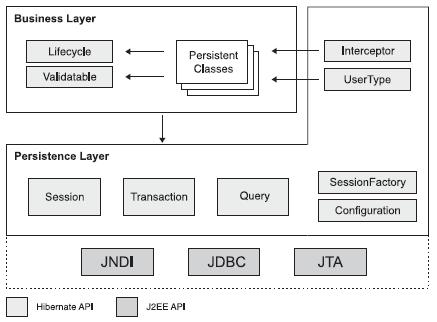
\includegraphics[scale=0.95]{images/Architektur-Hibernate.jpg}
	\caption{Architektur von Hibernate \citep[Bild 2.1]{Bauer2004}}
	\label{fig:architecture_hibernate}
\end{figure}

\vref{fig:architecture_hibernate} stellt die Rollen der wichtigsten Schnittstellen der Business- und Persistenzschicht von Hibernate dar. Dabei agiert die Businessschicht als ein Client der Persistenzschicht. In manchen Anwendungen werden diese beiden Schichten aber auch nicht getrennt dargestellt. Hibernate erm�glicht nach \citep{Bauer2004} auch die Verwendung von bestehenden Java APIs, wie z.B. JDBC, JTA oder JNDI. JDBC bietet abstrakte Funktionalit�ten analog zu relationalen Datenbanken und erlaubt es, fast jede Datenbank �ber einen JDBC Treiber mit Hibernate verwenden zu k�nnen. JNDI und JTA erm�glichen Hibernate die Integration in J2EE Applikationsservern.\\

�ber XML-basierte Mapping-Dateien wird das objektrelationale Abbilden der Java-klassen f�r Hibernate-Anwendungen definiert. Eine solche Mapping-Datei wird mit dem Dateinamen-Suffix \textit{.hbm.xml} versehen und wird generell f�r jede persistente Klasse erzeugt. In \vref{code:mapping_hibernate} wird das Prinzip der Mapping-Dateien dargestellt.

\begin{lstlisting}[language=XML, caption={Mapping-Datei von Hibernate}, label=code:mapping_hibernate, showstringspaces=false]
<hibernate-mapping>
  <class name="de.hsharz.provirent.objects.Bill" table="BILL">
	
    <id name="billId" type="int" column="BILLID">
      <meta attribute="scope-set">public</meta>
      <meta attribute="use-in-equals">true</meta>
      <generator class="native"/>
    </id>

    <many-to-one name="customer" class="de.hsharz.provirent.objects.Customer">
      <meta attribute="use-in-tostring">true</meta>
    </many-to-one>

    <property name="pdfFile" type="binary">
      <column name="pdffile" sql-type="BLOB" />
    </property>
				
    <property name="pdfFileSize" type="int">
      <meta attribute="use-in-tostring">true</meta>      	
    </property> 

  </class>
</hibernate-mapping>
\end{lstlisting}

In den Mapping-Dateien wird die Zuordnung der einzelnen Attribute (Properties) zu den entsprechenden Tabellenspalten der zugrunde liegenden Datenbank und auch Beziehungen zu anderen persistenten Java-Klassen (Relationen) festgelegt. Die folgende XML-Elemente sollten dabei verwendet werden:

\begin{itemize}

 \item class: Name der Java-Klasse und deren Zuordnung zur korrespondierenden Tabelle der Datenbank
 \item id: Attribut(e) der Klasse f�r den Prim�rschl�ssel
 \item property: Zuordnung der einzelnen Spalten der Datenbanktabelle zu den Properties der Java-Klasse mit zus�tzlichen Angaben �ber den zu mappenden Datentyp und das Erlauben von Null-Werten
 \item many-to-one: Darstellung einer n:1 Beziehung mit Zuordnung der Spalte aus der Datenbanktabelle zu einer entsprechenden Property und Angabe des Objekttyps der Beziehung

\end{itemize}

Au�er diesen gibt es noch weitere Attribute. �ber deren Bedeutung informieren die Hibernate-Webseiten.\\
Standardm��ig wird Hibernate �ber ein zentrales XML-Dokument konfiguriert. Der Name dieser Datei wird meist mit der Endung .cfg.xml gebildet. Darin werden solche Konfigurationen wie Deklaration der Datenbankverbindung, des Hibernate-Dialektes (abh�ngig vom verwendeten DBMS), sowie zus�tzlichen Optionen festgelegt. Ferner k�nnen auch die Ressourcen der einzelnen Mapping-Dateien angegeben werden, um diese der Java-Applikation bekanntzumachen.\\
Vor der Verwendung von Hibernate als Persistenzmechanismus in einer Anwendung muss die Hibernate-Umgebung initialisiert werden. Hierbei wird die Klasse \textit{SessionFactory} in der Gesch�ftslogik der Anwendung geladen. Mit Hilfe dieser Klasse l�sst sich eine Session-Instanz erzeugen, die als ein Bindeglied zwischen der Datenbank und der Anwendung fungiert. Nur �ber diese Session ist die Interaktion mit den Datenbankobjekten m�glich. Darunter sind die so genannten "`CRUD-Methoden"' (create, retrieve, update, delete) oder Queries (Abfragen mit HQL\footnote{Hibernate Query Language}) zu verstehen. \vref{code:save_hibernate} illustriert das Speichern des persistenten Objekts \textit{Dvd} in die Datenbank.\\

\begin{lstlisting}[language=Java, caption={Save-Methode der Hibernate-API}, label=code:save_hibernate, showstringspaces=false]
try {
  Dvd dvd = (Dvd) session.save(new Dvd());
} catch (HibernateException e) {
  logger.error("Objekt konnte nicht gespeichert werden", e);
}
\end{lstlisting}

Hibernate besitzt auch eine Transaktionsschnittstelle. So lassen sich �ber eine Transaktions-Instanz, die �ber das Session-Objekt erzeugt werden kann, Transaktionen durch geeignete Methoden (\textit{begin}/\textit{commit}/\textit{rollback}) abgrenzen. Diese Schnittstelle ist insofern erweiterbar, dass sie leicht mit anderen Systemen integriert werden kann. Weiterhin stehen dem Entwickler als Transaktionsstrategien sowohl optimistisches als auch pessimistisches Locking  zur Verf�gung.\\
Ein weiteres Merkmal von Hibernate ist die M�glichkeit der automatischen Generierung von Prim�rschl�sseln, wobei an die 10 verschiedenen M�glichkeiten, wie z.B. Sequenzen, im Vordergrund stehen.\\
Dar�ber hinaus stellt Hibernate verschiedene Abfragesprachen zur Verf�gung. Hierbei sind die Hibernate Query Language (HQL), Query By Criteria und Query By Example zu nennen. HQL ist an SQL angelehnt, beherrscht aber auch objektorientierte Konzepte wie Vererbung und Assoziationen. Die Anfragen werden dabei in Zeichenketten abgelegt und Hibernate �bergeben. Dieses Konzept l�sst sich in den Referenz-Dokumenten\footnote{siehe \citep{Hibernate2005}} von Hibernate  genauer betrachten. Bei der Verwendung von Query By Criteria werden keine Zeichenketten benutzt, sondern eine Anfrage setzt sich aus einzelnen Ausdr�cken zusammen, die zu einer so genannten \textit{CriteriaQuery} hinzugef�gt werden. Demnach wird die Syntax der Abfragen bereits zur �bersetzungszeit durch den Compiler und nicht erst zur Laufzeit �berpr�ft. Die Query By Example Schnittstelle nutzt das Konzept von Query By Criteria. Hierbei wird eine mit entsprechenden Suchdaten versehene Beispielklasse einer \textit{CriteriaQuery} �bergeben, woraufhin diese alle Klassen zur�ckliefert, die den Eigenschaften der �bergebenen Klasse entsprechen.























%Hier danach nicht mehr schreiben
\label{sec:tech-hibernate-ende}
%====================================
\chapter{Implementierung} \label{sec:Implementierung}


\chapter{Implementierung} \label{sec:Implementierung}
\section{Versionsverwaltung mit Subversion} \label{sec:impl-Versionsverwaltung}
Als Versionsverwaltung wurde Subversion verwendet. Dies hat mehrere Gr�nde: Zum einen war Subversion zu diesem Zeitpunkt eine neue und z.T. auch unbekannte Technologie, die somit ihren Reiz hatte. Zum anderen wurde Subversion als Nachfolger von CVS angepriesen und sollte viele Nachteile eliminieren. Einer der wichtigen Vorteile von Subversion ist die geringe Netzwerklast. Bei einem "`Commit"' werden nur die Unterschiede zur Vorg�ngerversion �bertragen und nicht wie bei CVS jede Datei komplett. Um Subversion verwenden zu k�nnen, wurde ein Rechner mit einem installieren Subversion Server ben�tigt, der m�glichst 24h im Internet verf�gbar ist. Um mit einem Client auf einen Subversion Server zuzugreifen, gibt es verschiedene �bertragungsprotokolle: Ein eigenes Subversion protokoll (svn), eine Kombination aus Secure Shell und dem eigenen Protokoll (ssh+svn), �ber http oder �ber https. Die sicherste Methode ist �ber ssh+svn, jedoch erfordert diese die Installation eines SSH Server, was unter Linux, dank verschiedener Anleitungen, einfach geht, jedoch unter Windows nicht so einfach zu realisieren ist. Unter Windows wurde zu Testzwecken ein Apache2 Webserver mit einem Zertifikat zur �bertragung von Daten per https installiert. Dieser Webserver wurde mit dem Subversion Server kombiniert und jeglicher Datentransfer f�r Subversion erfolgte �ber https und dessen eingestellen Port. Der Nachteil war jedoch, dass keiner die M�glichkeit hatte, einen PC 24h online zur Verf�gung zu stellen. So wurde nach einiger Suche im Internet der Open Source Anbieter Berlios Developer\footnote{\url{http://developer.berlios.de/}} entdeckt. Dort k�nnen Open-Source Projekte ihre Quellcodes in einer Subversion Versionsverwaltung mittels ssh+svn kostenlos speichern. Bei Berlios ist das Repository bereits erstellt, bei unseren Testsystem musste dies mit einem einfachen Befehl manuell erfolgen:
\begin{verbatim}
svnadmin create f:/subversion/phil/daten
\end{verbatim}
Durch diesen Befehl wurde in dem angegebenen Verzeichnis ein neues Repository erzeugt, das im Dateisystem auf dem Server die folgende Verzeichnisstruktur wie in \vref{fig:svnverzeichniss} zu sehen ist, erzeugt.
\begin{figure}[htbp]
	\centering
	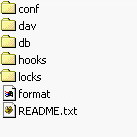
\includegraphics[scale=1.0]{images/svn-verzeichniss-struktur.jpg}
	\caption{Verzeichnisstruktur des Repository auf dem Server}
	\label{fig:svnverzeichniss}
\end{figure}
Im Verzeichnis \texttt{conf} befinden sich zwei wichtige Dateien. In der \texttt{svnserve.conf}, wie in \vref{code:svnserve} zu sehen, sind grundlegende Eigenschaften wie Zugangsberechtigungen, Begr��ung und Passwortdatei festgelegt. In der Passwortdatei, wie in \vref{code:svnuser} zu sehen, werden Benutzernamen und Passw�rter f�r die Benutzer dieses Repository vergeben. Diese Methode der Authentisierung ist jedoch nicht zu empfehlen, da die Passw�rter in dieser Datei lesbar sind und diese Datei, zus�tzlich zu anderen bereits vorhandenen Zugangslisten, aktuell gehalten werden muss.
\begin{lstlisting}[language=Java, showstringspaces=false, caption={Datei /conf/svnserve.conf},label=code:svnserve]
[general]
anon-access = none
auth-access = write
realm = Repository for my personal diplomarbeit
password-db = user
\end{lstlisting}
\begin{lstlisting}[language=Java, showstringspaces=false, caption={/conf/user},label=code:svnuser]
[users]
pschneider = geheim
\end{lstlisting}
Eine bessere M�glichkeit der Authentisierung w�re die �berpr�fung, bevor der Benutzer Zugang zum System erh�lt. Bei \emph{ssh+svn} erfolgt die Authensisierung durch ssh und bei https erfolgt diese �ber htaccess, in beiden F�llen wird dabei wahrscheinlich auf eine vorhandene Authentisierungsinfrastruktur zur�ckgegriffen.\\
\begin{figure}[htbp]
	\centering
	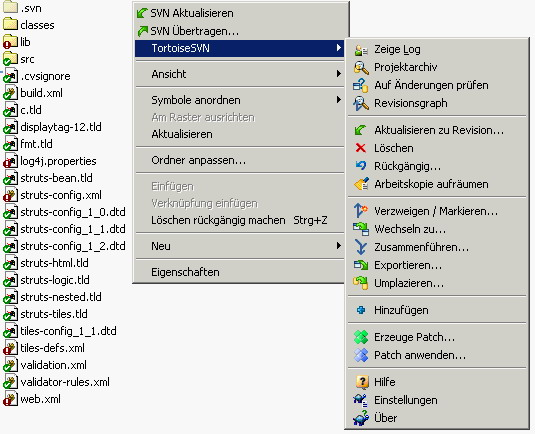
\includegraphics[scale=0.75]{images/svn-verzeichniss-client.jpg}
	\caption{Ansicht des Clients TortoiseSVN}
	\label{fig:svnclient}
\end{figure}
In unserem Projekt wurde als Client f�r den Zugriff auf das Subversionrepository TortoiseSvn\footnote{\url{http://tortoisesvn.tigris.org/}} verwendet. Dabei handelt es sich wie in \vref{fig:svnclient} zu sehen, um eine Windows-Shellerweiterung, die sich in den Explorer integriert. Ist ein Verzeichnis oder eine Datei Teil eines Projektes, das in einer Subversionversionsverwaltung gespeichert wird, sind diese durch kleine farbige Symbole markiert. Diese Symbole geben den Zustand der Dateien an, ob diese aktuell sind, ver�ndert wurden oder ob eventuelle Konflikte bestehen. Weiterhin k�nnen damit auch alle anderen Aktionen wie Log Datei betrachten, R�ckg�nging, Tagging/Merging und Verschiebungen wie in \vref{fig:svnclient} zu sehen, vorgenommen werden. Mit TortoiseSVN ist es auch m�glich nur ein bestimmtes Verzeichnis des meist sehr strukturiertes Projektes auszuchecken und zu bearbeiten. Dazu wird 
\texttt{TortoiseSVN $\Rightarrow$ Wechseln zu }, 
wie in \vref{fig:svnwechselnzu} zu sehen, ausgew�hlt. In dem sich �ffnenden Dialog wird das entsprechende Verzeichnis im Repository gew�hlt und die lokale Arbeitskopie wird automatisch auf die entsprechenden Verzeichnise und Dateien aktualisiert.\\
\begin{figure}[htbp]
	\centering
	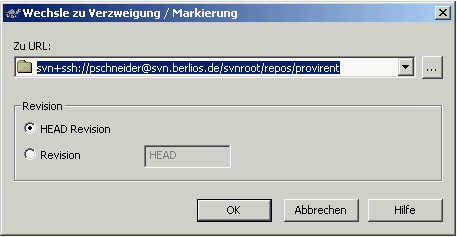
\includegraphics[scale=0.75]{images/svn-wechselnzu.jpg}
	\caption{Ansicht des Fensters zum wechseln der Arbeitskopie}
	\label{fig:svnwechselnzu}
\end{figure}
In den Einstellungen des Subversionservers k�nnen auch wie in \vref{tech-svn} bereits beschrieben, automatisch Email verschickt werden. Die in \vref{code:emailcommit} gezeigte Email soll verdeutlichen, welche Informationen mit diesem Mechanismus verschickt werden k�nnen. Im Betreff der Email befindet sich die neue Revisionnummer und das Verzeichnis in dem die �nderungen stattgefunden haben. Am Anfang der Email ist der Name des Authors, das Datum, eine Auflistung der ge�nderten Dateien und die Logmeldung zu sehen. Am Ende befinden sich die kompletten �nderungen als Text.


\begin{lstlisting}[language=Java, showstringspaces=false, caption={Auszug aus einer automatisch erzeugten Email},label=code:emailcommit]
Author: rgriesch
Date: 2005-12-02 21:04:22 +0100 (Fri, 02 Dec 2005)
New Revision: 276

Modified:
   project_src/provirent_hibernate/src/de/hsharz/provirent/management/gui/ManagementGui.java
Log:
Menu Rechnung fehlt  - sollte aber aus Zeitgr?\195?\188nden                                nicht mehr implementiert                                   werden !!
ManagementGui        - Reiter Film war aktiv, obwohl
                       Fenster kunden angezeigt wurde
                       ( Fehler behoben )
ManagementGui        - Button Beenden im Menu "Datei"
                       wurde Funktionalit?\195?\164t eingef?\195?\188gt   

Modified: project_src/provirent_hibernate/src/de/hsharz/provirent/management/gui/ManagementGui.java
===================================================================
--- project_src/provirent_hibernate/src/de/hsharz/provirent/management/gui/ManagementGui.java	2005-11-30 15:04:55 UTC (rev 275)
+++ project_src/provirent_hibernate/src/de/hsharz/provirent/management/gui/ManagementGui.java	2005-12-02 20:04:22 UTC (rev 276)
@@ -412,9 +412,12 @@
 
 		exitMenuItem = new MenuItem(fileMenu, SWT.CASCADE);
 		exitMenuItem.setText(l.getString("menu.file.exit"));
-
+		exitMenuItem.addSelectionListener(new SelectionAdapter() {
+			public void widgetSelected(SelectionEvent evt) {
+			    shell.close();
+			}
+		});
 	}
-
 	/**
 	 * init the View Menu
 	 */
@@ -484,7 +487,7 @@
 
 		viewCustomerMenuItem = new MenuItem(viewMenu, SWT.CHECK);
 		viewCustomerMenuItem.setText(l.getString("menu.view.customer"));
-		viewCustomerMenuItem.setSelection(false);
+		viewCustomerMenuItem.setSelection(true);
 		viewCustomerMenuItem.addSelectionListener(new SelectionAdapter() {
 			public void widgetSelected(SelectionEvent evt) {
 				if (tabItemCustomer == null || tabItemCustomer.isDisposed()) {
@@ -599,7 +602,7 @@
 
 		viewMovieMenuItem = new MenuItem(viewMenu, SWT.CHECK);
 		viewMovieMenuItem.setText(l.getString("menu.view.movie"));
-		viewMovieMenuItem.setSelection(true);
+		viewMovieMenuItem.setSelection(false);
 		viewMovieMenuItem.addSelectionListener(new SelectionAdapter() {
 			public void widgetSelected(SelectionEvent evt) {
 				if (tabItemMovie == null || tabItemMovie.isDisposed()) {

_______________________________________________
Provirent-svn-commit mailing list
Provirent-svn-commit@lists.berlios.de
http://lists.berlios.de/mailman/listinfo/provirent-svn-commit
\end{lstlisting}















%Hier danach nicht mehr schreiben
\label{sec:impl-Versionsverwaltung-ende}

%\section{Entwicklungsumgebung mit Eclipse}


\section{grafischen Benutzerschnittstellen mit SWT} \label{sec:impl-Benutzerschnittstellen}
\section{Java-Web-Anwendungen mit Struts} \label{sec:impl-WebAnwendungen}



















%Hier danach nicht mehr schreiben
\label{sec:impl-WebAnwendungen-ende}
\section{Persistenzschichten mit Hibernate} \label{sec:impl-Persistenzschichten}

Die Implementation der Persistenzschicht unter Verwendung von Hibernate



















%Hier danach nicht mehr schreiben
\label{sec:impl-Persistenzschichten-ende}
%====================================
\chapter{Fazit} \label{sec:Fazit}
Mit Hilfe dieses Projektes wurde bei allen Projektmitglieder Erfahrungen im Bereich Softwareplanung und Softwareentwicklung gesammelt. Bei diesem Projekt wurde eine eigenst�ndige Idee in die Realit�t umgesetzt, wobei alle Projektmitglieder dabei intensiv und mit viel Interesse an einer m�glichst guten Realisierung mitarbeiteten.\\

Technologisch gesehen haben sich die Projektmitglieder in Themengebiete gewagt, die ihnen bis dahin zum Teil relativ fremd waren. So wurden im Bereich vom objektrelationalen Mapping �berhaupt die ersten Erfahrungen gesammelt. Dazu wurde die Erkenntnis gewonnen, dass Hibernate ein sehr vorteilhaftes und umfassendes Werkzeug ist, um die Persistenzschicht von der Businessschicht unabh�ngig zu gestalten.\\
So wurde erreicht, dass diese Persistenzschicht vollst�ndig implementiert werden konnte und f�r den Zugriff aus dem Kundenmodul und dem Verwaltungsmodul zur Verf�gung steht.\\

Weiterhin ist festzustellen, dass die Implementierung des Projekts noch nicht abgeschlossen ist, so dass z.B. noch grundlegende Funktionalit�ten des Kundenmoduls umgesetzt werden m�ssen. Trotzdem konnte und kann hier die Verwendung des Webframeworks Apache Struts dazu beitragen, dass mit relativ wenig Aufwand und Entwicklungszeit die Entwicklung einer 3-schichtigen Webanwendung erm�glicht wird. Dies hat den Vorteil, dass Design, Businesslogik und Daten von einander getrennt dargestellt und umgesetzt werden konnten.\\

Durch die Verwendung von Subversion als Versionsverwaltung wurde der Umgang mit einer neuen Technologie schnell zur Gewohnheit. Dadurch ist es f�r die Projektmitglieder zum Alltag geworden, �nderungen sofort f�r alle zu speichern und mit aussagekr�ftigen Kommentaren zu versehen. Durch die netzwerksparende �bertragung von Daten, war auch der Einsatz von Modems m�glich. Durch den  automatischen Versand von Emails wurden andere Projektmitglieder schnell und kompakt �ber �nderungen informiert. Die installation auf einem Windowstestrechner mit einer gesicherter HTTPS-Verbindung gestaltete sich als unkompliziert, wie die Installation einer gesicherten ssh+svn Verbindung auf einem Fedore Core 3 Linux Rechner, dank gut beschriebener Anleitungen.\\

Aufgrund der SWT-Bibliothek konnte eine einfach zu bedienende Benutzeroberfl�che erstellt werden, mit der alle notwendigen Objekte f�r eine Online-Videothek einfach editiert und erstellt werden k�nnen. Aufgrund der verwendeten Reiter f�r jedes Untermen� kann schnell zwischen den einzelnen Men�s umgeschaltet und Ver�nderungen vorgenommen werden. Die verschiedenen Dialogfenster erleichtern die Eingabe f�r den Benutzer und zugleich die Bearbeitung im Quellcode.\\

Dieses Projekt k�nnte auch als Grundlage f�r andere Studentenprojekte dienen. Dabei m��en die Studenten sich nicht in dieses spezielle Projekt einarbeiten, sondern k�nnen ein selbst�ndiges Modul entwickeln. So k�nnten Studenten bspw. ein Suchmodul mit Apache Lucence entwickeln oder ein Barcodemodul zur Verarbeitung von Barcodes entwickeln. Weiterhin k�nnte ein Modul zur Erstellung von Rechnungen oder anderen Reports mit Eclipse Birt erstellt werden, ein Modul zur Verwaltung der Standorte/Lagerorte der DVD's oder ein Modul zur Berechnung der k�rzesten Wegstrecke bei der Zusammenstellung einer bzw. mehrerer Bestellungen. Jedes dieser Module k�nnte dann mit geringen Aufwand in die Online-Videothek integriert werden.




\label{sec:Fazit-ende}


%====================================
\chapter{Zusammenfassung} \label{sec:Zusamenfassung}





\textbf{\emph{Hier muss beschrieben werden, was in den einzelnen Abschnitten beschrieben wurde.}}
%====================================


\appendix
\chapter{Protokoll vom 11. Mai 2004}

Drei Frameworks stehen zur Auswahl \\
\begin{itemize}
	\item Apache Cocoon
	\item Apache Struts
	\item Apache Tapestry
\end{itemize}

Jeder erstellt eine einfache (Web)Anwendung mit Hilfe eines dieser Frameworks 
folgende Komponenten sollen/muessen enthalten sein: \\
\begin{itemize}
	\item einfache LoginSeite (�ber Datenbank)
	\item Liste aller Videos in Datenbank anzeigen
	\item EingabeMaske f�r neues Labor
	\item Validierung der Eingabedaten
	\item dynamische Navigation
	\item eventuell ein Bild f�r den Status der einzelnen Bilder (dynamisches Bild??)
\end{itemize}

F�r diese BeispielAnwendung sollen m�glichst viele Elemente des jeweiligen Framework verwendet werden.
Wichtig ist dabei der Umgang und die Bedienbarkeit des Systems. \\
Wiederverwendbarkeit einzelner Module. \\
Design und Logik Trennung vorhanden? Kann das Design einfach/schnell ausgetauscht werden.\\
\\
Es geht dabei nicht um ein 100% fehlerfreies System.\\
Design spielt keine wichtige Rolle, es sollte jedoch beachtet werden, dass dieses sp�ter vom Kunden ausgetauscht werden m�chte.\\
\\
\\
\begin{itemize}
	\item Struts: Stefan
	\item Cocoon: Philipp
	\item Tapestry: Remo
\\
	\item Namen f�r das Projekt finden
	\item Link mit Beispiel Webseiten rumschicken
\end{itemize}
	
%%%%%%%%%%%%%%%%%%%%%%%%%%%%%%%%%%%%%%%%%%%%%%%%%%%%%%%%%%%%%%%%%
% 																															%
%---------------------------------------------------------------%
%                         9-1Literatur.tex                      %
%%%%%%%%%%%%%%%%%%%%%%%%%%%%%%%%%%%%%%%%%%%%%%%%%%%%%%%%%%%%%%%%%

%\nocite{Wessel2005}
\addcontentsline{toc}{chapter}{Literaturverzeichnis}
\bibliography{Provirent-Doku}
%%%%%%%%%%%%%%%%%%%%%%%%%%%%%%%%%%%%%%%%%%%%%%%%%%%%%%%%%%%%%%%%%%
% 																															%
%---------------------------------------------------------------%
%            9-2Abkuerzungsverzeichnis.tex                      %
% Abk�rzungen sp�ter in den Text direkt uebernehmen, dort wie diese das erste mal verwendet werden, somit 
% kann mittels refpage auf die Seite verwiesen werden
%%%%%%%%%%%%%%%%%%%%%%%%%%%%%%%%%%%%%%%%%%%%%%%%%%%%%%%%%%%%%%%%%
\addcontentsline{toc}{chapter}{Abk�rzungsverzeichnis}


\printnomenclature
%\addcontentsline{toc}{chapter}{Index}
%\printindex
%%%%%%%%%%%%%%%%%%%%%%%%%%%%%%%%%%%%%%%%%%%%%%%%%%%%%%%%%%%%%%%%%%
% 																															%
%---------------------------------------------------------------%
%                        9-2Erklaerung.tex                      %
%%%%%%%%%%%%%%%%%%%%%%%%%%%%%%%%%%%%%%%%%%%%%%%%%%%%%%%%%%%%%%%%%
\addcontentsline{toc}{chapter}{Erkl�rung}
\chapter*{Erkl�rung}

\vspace*{2cm}
Ich erkl�re hiermit, dass ich zur Anfertigung der vorliegenden Arbeit keine anderen als die angegebenen Quellen und Hilfsmittel und keine nichtgenannte fremde Hilfe in Anspruch genommen habe. Mir ist bewusst, dass eine falsche Versicherung rechtliche Konsequenzen hat.

\vspace{4cm} Leipzig, den \today  \\





%------ Ende des Dokumentes ------
\end{document}